\documentclass[
	%parspace, % Add vertical space between paragraphs
	%noindent, % No indentation of first lines in each paragraph
	%nohyp, % No hyphenation of words
	%twoside, % Double sided format
	%draft, % Quicker draft compilation without rendering images
	%final, % Set final to hide todos
]{elteikthesis}[2024/04/26]

% The minted package is also supported for source highlighting
% See elteikthesis_minted.tex for example
%\usepackage[newfloat]{minted}

% Document's metadata
\title{Myocardial Perfusion Imaging using Vision Transformers} % title
\date{2025} % year of defense

% Author's metadata
\author{Haris Ali}
\degree{Computer Science MSc}

% Superivsor(s)' metadata
\supervisor{Szűcs, Ádám István} % internal supervisor's name
\affiliation{PhD Candidate} % internal supervisor's affiliation
%\extsupervisor{Jane Doe} % external supervisor's name
%\extaffiliation{Senior Developer} % external supervisor's affiliation

% University's metadata
\university{Eötvös Loránd University} % university's name
\faculty{Faculty of Informatics} % faculty's name
\department{Dept. of Artificial Intelligence.} % department's name
\city{Budapest} % city
\logo{elte_cimer_szines} % logo

% Add bibliography file
\addbibresource{elteikthesis.bib}

% The document
\begin{document}

% Set document language
%\documentlang{hungarian}
\documentlang{english}

% List of todos (not in the final document)
%\listoftodos[\todolabel]

% Title page (mandatory)
\maketitle
% Topic declaration page (mandatory) - can also be attached instead
%\includepdf{topicdeclaration.pdf}

\chapter*{Declaration}
\addcontentsline{toc}{chapter}{Declaration}

I hereby declare that this thesis titled “Myocardial Perfusion Imaging with Vision Transformers” and the work presented in it is my own original research. I confirm that:

\begin{itemize}
    \item This work was done wholly or mainly while in candidature for a research degree at Eötvös Loránd University.
    \item Where I have consulted the published work of others, this is always clearly attributed.
    \item Where I have quoted from the work of others, the source is always given.
    \item I have acknowledged all main sources of help.
    \item This thesis has not been submitted for any other degree or professional qualification.
\end{itemize}

\vspace{1cm}
\noindent
Signed: Haris Ali \\
\vspace{0.2cm}
Date: 13th April, 2025


\chapter*{Acknowledgements}
\addcontentsline{toc}{chapter}{Acknowledgements}

I would like to express my sincere gratitude to my supervisor, \textbf{Szűcs, Ádám István}, for his continous support and guidance throughout this research. His expertise were extremely valuable for the development of the project and reach it to completion.

I am also thankful to the faculty and staff of the Department of Computer Science at Eötvös Loránd University, whose valuable support were crucial for the carrying out of the research.

Lastly, I appreciate the open-source community and all the developers whose tools and libraries played a significant role in the implementation of this project.

\vspace{0.5cm}
\noindent
Thank you all.

\cleardoublepage

% Table of contents (mandatory)
\tableofcontents
\cleardoublepage

% Main content
% Abstract (mandatory)
\chapter*{Abstract}
\addcontentsline{toc}{chapter}{Abstract}

The manual delineating the left ventricle (LV) in Myocardial Perfusion Imaging (MPI) is one of the most labour-intensive and time consuming tasks in nuclear cardiology and radiology. The outcome of the diagnosis of the MPI is extremely dependent on the accuracyand the consistency of the segmentation of the ventricles, hence the process is done under extreme caution in roder to minimize the risks of any possible error. However, the process of turning this task into an automated one present a number of challenges that need to bbe mitigated. Fist of all, the signal-to-noise ration (SNR) is mostly low and the resolution of the image is limited, complicating the process of detecting the boundaries. Secondly, the high disparity in both the cardiac traces uptake ad the differences in the hardware used for the imaging introduces inconsistencies. Finally, their is a lack of a standardized definition of the shape of the LV and the there is no standard shape that can be traced based purely on image data, which introduces a lot more ambiguity in the task.

This thesis proposes a novel method built to address the limitations mentioned above by using a Transformer-based architecture, integrating statistical shape prior (SSP) technique. This approach is specifically used to mitigate the data-hungry nature of the transformers in case of limited deta. The proposed architecture achieves over 4\% improvementover a number of metrics in segmentation and classification against the benchmarked state-of-the-art (SOTA) approaches use for LV segmentation, both on the synthetic data and the real-world clinical scans.

In addition to the improvements in the quantitative metrics, the incorporation of the prior shape information enabled the model to learn insights into the variability and the structural patterns of the LV anatomy in MPI single-photon emission tomography (SPECT) imaging. This deeper understanding of the LV enhances the reliability of the AI-powered automatic segmentation of the LV and also the general comprehension of the morphology of the LV in clinical practice.
\cleardoublepage

\chapter{Introduction}
\label{ch:intro}

Myocardial Perfusion Imaging (MPI) using single-photon emission computed tomography (SPECT) pllays an important role in the process of non-invasive assessment of the coronary artery disease (CAD). Considering cardiovascular diseases being one of the leading causes of mortality all across the world, the need for an efficient, accurate and accessible tool for diagnosis is at a high demand. MPI SPECT provides critical information about the perfusion status of the heart, which helps in the early detection and planning the treatment which improves the outcomes of the patients.

Radionuclide MPI under a specific condition, such as stress, is majorly regarded as one of the most effective diagnosis technique, which is also non-invasive, in order to identify the or detect the coronary artery disease (CAD). Using the application of MPI SPECT, clinicians become equipped to diagnose and detect the functionally relevant coronary stenoses with a relatively high level of specificity This actually enables them to make decisions that are informed and possibly the right ones regarding the pathways of the patients' treatment \cite{10.1001/jamacardio.2017.2471}. By visualizing the perfusion process of the heart muscles, clinicians can detect the areas of the heart where there is a presence of coronary stenoses or obstructions which may be the causing issue for inducible perfusion deficits under the conditions of stress or rest. This ability of diagnosis is not only essential to identify the patients with CAD but also functions as an important tool for mitigating patient risk and guiding the decision making process of the clinicians.

MPI using SPECT has emerged as both an effective and economically viable modality for the purpose of diagnosis. MPI based SPECT offers both the advantages of being accessible and having established standard clinical protocols hence it is the preferred choice of a number of diagnostic processes. One of the major strengths of MPI is the adaptability of the technique, as it can incorporate a number of radio-pharmaceutical agents, such as 201Tl Chloride, 99mTc Tetrofosmin, and 99mTc Sestamibi, which basically is dependent upon the imaging protocols and imaging needs. The mentioned agents are typically administered intravenously before the image acquisition part, and then the collected image data are later reconstructed using techniques which are dedicatedly designed for cardiac imagery. The last, and possibly the most crucial, stages in the diagnostic process involves the segmentation of the anatomical structures relevant to the diseases and then the reorientation of this segmented volumetric data. This part of the diagnostic is usually performed by trained clinical professionals in order to ensure precision, better reliability and to mitigate the risks of errors.

Beyond the usage of the perfusion imaging alone, there are additional functional parameters, which are valuable, that can be derived when gated acquisition techniques are applied. These parameters include end-systolic volume (ESV), end-diastolic volume (EDV), and the left ventricular ejection fraction (LVEF). All of the mentioned parameters are essential in order to indicate the performance of the heart. The values of these parameters are computed through the precise delineation of the myocardial boundaries of the LV,, which makes the task of segmentation even more crucial in the whole pipeline. The perfusion and the functional analysis collectively provide a detailed understanding of not only the vascular but also the mechanical health of the heart.

Efficient and accurate quantitative analysis of the 3D MPI SPECT data is extremely sensitive to a number of factors that are involved in the full end-to-end imaging and reconstruction pipeline, as mentioned above. All of these factors together contribute not only to the reliability of the evaluation of the data, but also to the detection of a range of cardiac abnormalities \cite{SLOMKA2012338}. The important step in this process is the segmentation and reorientation of the LV, which basically refers to the determination of the spatial alignment of the LV and its segmentation based on the anatomical midline. The tasks of both reorientation and the segmentation within MPI SPECT imaging have been acknowledged, for a long time, as one of the central yet difficult challenges. Over the course of years, multiple commercial systems have been developed in order to counter these issues, but more often relying on very extensive and curated datasets in order to ensure reliable performance in clinical environments \cite{Garcia2007}, \cite{Liu2007}, \cite{Ficaro2007}.However, the existing solutions fall short when they are applied to the newer reconstruction paradigms, especially in the situations where there are only a limited number of labled patients datasets. In order to mitigate these imitations faced by the current solutions and to increase the generalization capabilities of the models under limited data conditions, approaches incorporating self-supervised learning and few-shot learning have gained popularity. Nevertheless, the effectiveness of these strategies is most of the times overshadowed by the high costs associated with the expert annotations. In addition to this the lack of consensus regarding a standard segmentation protocol also complicate the practical application of the processes.

In the recent years, within the field of MPI SPECT imaging, the adoption of Deep Learning (DL) techniques are looking at a significant revival \cite{tolu2025advancements}. This renewal is basically driven in part by the development of the novel radio-tracers and also the growing clinical demand to minimize the amount of administered radiation dose and also the image acquisition time of the performed procedures \cite{henzlova2011future}. As a consequence, the modern methods of reconstruction have been focusing on configurations that are based on low photon count data, sparse acquisition views and reduced amount of injected doses \cite{xie2023transformer}, \cite{xie2024generalizable}, \cite{chen2024dudocfnet}. But in-spite all that, the advancements do not fully resolve the challenges which are inherent to the segmentation tasks of MPI SPECT. Despite using state-of-the-art neural network based reconstruction strategies, the segmentation accuracy is still heavily relied on the underlying reconstructed images. When working with lower-dose inputs, the images mostly lack proper structural clarity, which diminishes the benefits which are offered by the DL based reconstruction methods. Even in situations where the image reconstruction achieves are visual equivalence to a full-dose filtered back projection methods, the issues of low Signal-to-Noise Ratio (SNR), Poisson noise characteristics, and the impact of partial volume effect (PVE) continue to affect the generalization capabilities and hence the reliability of automated segmentation models.

In this work, is proposed a novel approach in order to solve the aforementioned bottlenecks of the segmentation task, all the while also contributing further detailed insights into the anatomical characteristics of the MPI SPECT LV. Contrary to the previous approaches employed for the task, where the use of isolated pre-processed regions, or usage of cropped volumes, is common, the method in this study makes use of the entire reconstructed image volumes, hence incorporating all of the contextual spatial cues which are available within the full field-of-view (FOV). The choice of this design makes sure that no information that is diagnostically relevant is discarded, hence allowing the model to infer the left ventricular structure in relations to the surrounding regions of the anatomy. This holistic approach increases the robustness of the model, specifically in cases where abnormalities in the patterns could possibly interfere with the more localized analysis.

In order to mitigate the limitations hat are associated with convolutional neural networks (CNN), specifically their receptive field being restricted which hinders them from learning long-range dependencies, the proposed method employs a fully transformer based architecture called nnFormer \cite{zhou2023nnformer}. This architecture is specifically developed for tasks pertaining to volumetric medical imaging. It allows the network to learn global reasoning over the 3D structures which offers a significant advantage over the traditional CNNs in situations where the boundaries of the organs are not sharply defined such as SPECT. But there is a limitation to using transformer architectures, which is that they require a huge amount of data in order to learn acceptable global representations and have a good generalization ability. Hence, in order to overcome such a limitation, the proposed method incorporates Statistical Shape Priors (SSP) as a regularization technique. Such shape priors introduce an anatomical consistency into the DL model which acts as a guidance signal during the training of the model. This approach helps the models in situations where the amount of available data is limited. Using the shape priors, the model is made to learn meaningful and spatially coherent segmentation outputs even with minimal amount of supervision. This whole process bridges the gap between the traditional rule-based segmentation models and the fully data driven DL approaches.

\cleardoublepage

\chapter{Methodology}
\label{ch:method}

\section{Overview}
The main goal of the research is to propose a comprehensive and strong method which is designed specifically to significantly improve the accuracy of the segmentation of \gls{mpi} using \gls{spect} for the \gls{lv}. The precise segmentation of \gls{mpi} \gls{spect} images is extremely critical for the detection and the assessment of \gls{cad}. However, the task of achieving a high accuracy in segmentation poses a number of challenges due to a multitude of inherent limitations of \gls{mpi} \gls{spect} data, such as low \gls{snr} partial volume affects, substantial noise because of the Poisson statistics, motion artifacts and, obviously, the anatomical variability among different patients. 

In order to address these challenges, the proposed research amalgamates advanced approaches in the field of \gls{dl}, more specifically utilizing the transformer based architecture known as nnFormer \cite{10.1109/TIP.2023.3293771}, which is combined with an innovative idea of using \gls{ssp}s. The nnFormer architecture is chosen because of the ability of it of capturing both the local and the global information or contextual relationships in volumetric data as opposed to traditional CNNs which only capture local information. nnFormer leverages the \gls{lvmsa} and the \gls{gvmsa} mechanisms very efficiently in a unified method. These modules of the transformer architecture very effectively encode the long-range dependencies which are extremely important for better segmentation accuracy specifically in medical imaging where they are characterized by indistinct boundaries.

Simultaneously, the \gls{ssp} are merged into the segmentation pipeline in order to improve the anatomical consistency of the model. SSPs provide the \gls{dl} model with a mathematical model which captures the probabilistic variability off the \gls{lv} that are derived from the data annotated by experts. This \gls{ssp} methods employs an advanced technique of optimization such as Mahalanobis distance based regularization and the Kullback-Liebler (KL) divergence in order to refine the segmentation boundaries. This way the outputs of the segmentation model maintain plausible anatomical outputs, which improves the segmentation accuracy even when the input data is incomplete or ambiguous. The combination of nnFormer and \gls{ssp} provides us with a novel hybrid architecture. The full architecture pipeline is presented, on an abstract level, in \cref{Fig:network_pipeline}.

This hybrid approach leverages not only the strengths of \gls{dl} models in extracting complex and hierarchical feature representations from volumetric data, but also the advantages of SSPs in maintaining consistent anatomies. This approach also addressees the limitations of the existing methods, which include inefficient generalization capability and dependencies of large, precisely annotated data for training. It also mitigates the impact of a number of different imaging artifacts and the noise, which enhances the overall reliability on the segmentation.

Extensive procedures for training involving efficient optimization strategies such as Adam, and specifically segmentation tailored loss such as the DiceCELoss, are implemented in order to ensure stable performance across a diverse set of patients. The training and the validation aspects are conducted rigorously using an extensive dataset of \gls{mpi} \gls{spect} which consists of diverse collimation methods and demographics of the patients which improves the generalization capability of the method. Extensive setups of computation which leverage high performance GPU computing environments ensure efficient training and inference of the model. Comprehensive evaluation metrics are utilized in order to quantitatively validate the performance of the segmentation. These metrics include precision, recall, intersection over union (IoU) and Dice coefficient. These metrics provide an extremely in-depth insights into the capability of the method to handle real-world variability and complex scenarios.

In a summary, the proposed methodology contributes to not only a significant advancement in the division of cardiac image segmentation but also provides a practical and robust solution which is applicable in a clinical environment. The combination of nnFormer and \gls{ssp} ensures reliable and precise segmentation having clinically meaningful results, which paves the way for better and improved diagnosis and patient outcomes in \gls{cad} management.

\begin{figure}[htb!] % Changed from figure* to figure unless you specifically need double-column
\centering
% \begin{subfigure}[b]{1.5\textwidth} 
\centering
\resizebox{1\textwidth}{!}{

\begin{tikzpicture}[
    node distance=8mm and 0mm,
    block/.style={draw, fill=blue!10, rounded corners, minimum width=3cm, minimum height=1cm, align=center},
    arrow/.style={-Stealth, thick},
    shapenode/.style={ellipse, draw, fill=red!10, minimum width=2cm},
    legendbox/.style={draw, fill=white, font=\small}
]

% Input
\node (input) {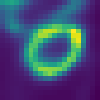
\includegraphics[width=1.2cm]{sagittal_input.png}};
\node[above=1mm of input, font=\footnotesize] {Input SPECT Volume};

% Preprocessing
\node[block, below=of input] (preprocess) {Preprocessing \\ (Normalization, Denoising)};
\draw[arrow] (input) -- (preprocess);

% Shape Prior Path
\node[shapenode, left=of preprocess, xshift=-1cm] (shape) {Statistical Shape Model};
% \draw[arrow] (shape) -- (priors);
% \draw[arrow, dashed] (input.west) -- ++(-6cm,0) |-  (shape.north);
% \draw[arrow, dashed] (input.west) -- ++(-6cm,0) coordinate (temp) -- (temp|-shape.north) -- (shape.north);
\coordinate (temp) at ($(input.west) + (-6.05cm, 0)$);
\coordinate (drop) at ($(shape.north) + (-0cm, 0.1)$);

\draw[arrow, dashed] (input.west) -- (temp) -- (drop) -- (shape.north);


% Transformer Encoder
\node[block, below=of preprocess] (encoder) {nnFormer Encoder};
\draw[arrow] (preprocess) -- (encoder);
% \draw[arrow, dashed] (shape.east) -- (preprocess.west);

% Fusion
\node[block, below=of encoder] (fusion) {Feature Fusion \\ (nnFormer Features \ensuremath{\oplus} Shape Priors)};\draw[arrow] (encoder) -- (fusion);
\draw[arrow] (shape.south) |- ([xshift=-5mm]fusion.west) -- (fusion.west);

% Decoder
\node[block, below=of fusion] (decoder) {nnFormer Decoder};
\draw[arrow] (fusion) -- (decoder);
\draw[arrow, dashed] (encoder.east) -| ++(2cm,0) |- (decoder.east);

% Output
\node[below=of decoder] (output) {
\includegraphics[width=1.2cm]{sagittal_gt.png}};
\node[below=1mm of output, font=\footnotesize] {LV Segmentation Mask};
\draw[arrow] (decoder) -- (output);


% Ensure all content is within bounds
\useasboundingbox (current bounding box.south west) rectangle ([xshift=6cm]current bounding box.north east);

\end{tikzpicture}
}
\caption{\centering Network architecture pipeline}
\label{Fig:network_pipeline}
\end{figure}

\section{Data Acquisition and Preprocessing}

The \gls{mpi} dataset which is utilized in this research was acquired using \gls{spect}. This acquired dataset consists of volumes from a total of 80 patients, which are carefully selected in order to represent the diverse demographic and the characteristics of the clinic. The population of the patients included individuals with varying age groups, physiological conditions and gender distributions in order to ensure the reliability, robustness and generalizability of the model. Multiple different radio-tracers were employed in the process of acquiring the \gls{mpi} \gls{spect}, specifically agents labled by technetium-99m(Tc) such as Tc Tetrofosmin and TC Sestamibi, and also the thallium 201 chloride (T1 Chloride). Each of these radio-traces offer unique properties in imaging thereby providing a comprehensive coverage of all the possible clinical scenarios which are encountered in everyday diagnostic. 

The dataset of the patients used in the research is divided into five distinct groups. \textbf{(A)} The first, and the largest group is a heterogeneous black-box dataset which comprises of patients who are scanned under multiple d efferent geometries, pharmaceutical protocols and the settings of the acquisition. This group consisted of 40 individuals, out of which 27 were female and 13 male with an average age of 69.62 years. The average height of the group is 167.25cm while the average weight is 78.11 kgs. \textbf{(B)} The second group consists of 10 patients who are imaged using the most recent MPH collimator configurations,, specifically the APT73 collimators installed on the Mediso AnyScan Trio system. This group consists of 7 females and 3 males with an average age of 68.8 years, an average height of 169 cm, and an average weight of 73.8 kgs. \textbf{(C)} The third group comprises of another 10 patients scanned with the LEHR-HS collimator which is also mounted with a trio camera. Out of these, 8 are female and 2 male with an average age of 68 years, an average height of 176 cm and an average weight of 92 kgs. \textbf{(D)} the fourth group was scanned using the earlier generation imaging hardware, in order to provide a comprehensive basis with the legacy systems. This group included data from 10 patients who are scanned using the Mediso CardioD system in a seated configuration setting. This group consisted of 1 female and 9 male subjects with an average age of 75.6 years, an average height of 151 cm and a mean weight of 71 kgs. \textbf{(E)} The fifth and last group also involved 10 individuals who are imaged with the Mediso CardioC system with subjects positioned supine. This group consists of 7 females and 3 males. The retrospective nature of this dataset is stored in the interfile format due to format limitations and only the average age could be reliably extracted which comes out ot be 70.33 years.

Each of the patient went through very rigorous imaging procedures which are adhering strictly to standard protocols of acquisition in clinics. The patients were administered the mentioned radio-pharmaceuticals intravenously which was followed by image acquisition after the standardized waiting period that allows sufficient tracer uptake in the myocardial tissue. The image acquisition protocols were varying based on the collimation method which was employed. For example imaging with the MPH collimator a very specific step-and-shoot helical trajectories, on the other hand the stationary collimator positions were employed for the other collimators which creates different spatial sampling patterns and different challenges to image reconstruction. After the acquisition of the raw data, a number of precprocessing techniques were employed in order to prepare the data for the subsequent segmentation analysis. The preprocessing pipeline was developed in order to address a number of inherent issues with the imaging and to optimize the data quality for better segmentation outcomes.

The preprocessing steps began with the correction of the attenuation utilizing the TeraTomo reconstruction algorithm \cite{Nagy2013}, which majorly removed the attenuation artifacts which are caused by the soft bone and tissue structures. This step is very essential in order to ensure the uniformity in the distribution representation of the tracer across the myocardial tissue, hence improving the segmentation accuracy. In some cases where the attenuation correction data was not available, an Ordered Subset Expectation Maximization (OSEM) algorithm \cite{Hudson1994} was used in order to reconstruct the full \gls{fov} volumes, providing us with data with robust handling of Poisson noise and preserving essential details of the image. 

In order to improve the image quality even more, noise reduction techniques are employed, specifically targeting the reduction of the Poisson noise which is the most prominent in \gls{mpi} \gls{spect} imaging due to the low count of the photons. More advanced filtering methods were also employed such as the Gaussian smoothing and the adaptive median filtering in order to balance the noise reduction with the preservation of important boundaries anatomically and the structural details. The partial volume effects (PVE), which majorly has an impact on the accuracy of the segmentation because of blurring tissue boundaries, were addressed systematically using dedicated PV correction techniques and de-convolution techniques. These methods restored the sharpness in the images and enhanced the delineation of th myocardial boundaries, especially in the regions which have complex anatomical structures.

The images that are the result of the above preprocessing are made to go through further normalization procedures in order to ensure consistency in the scales of intensity across all the datasets which helps in having more robust training of the final segmentation models. Standardization of the intensities of the voxels involved scaling the pixel intensity distribution in order to have a mean of zero and a unit variance, which significantly improves the numerical stability, which in-turn helps the convergence of the \gls{dl} models.

All the data preprocessing steps are performed in a very structured and repeatable framework, using scripts that are custom developed in Python and specialized libraries for numerical computation, imaging and \gls{dl} such as PyTorch \cite{NEURIPS2019_9015}, NumPy \cite{harris2020array} and Scikit-learn \cite{pedregosa2011scikit}. The comprehensive documentation of the preprocessing parameters and the configurations was nicely maintained so as to ensure the transparency and the reproducibility of the methodology. The final dataset after the preprocessing provided us with a very high-quality and standardized input data for the training, validation and the testing of the \gls{dl} models. The careful handling of the whole data acquisition pipeline ensuring the variability and the rigorous preprocessing ensured optimal \gls{mpi} \gls{spect} image preparation which majorly enhanced the accuracy and the reliability of the segmentation which was obtained from the hybrid model.

\section{Detailed Description of nnFormer Architecture}

The nnFormer architecture introduces an innovative advancements in the field of medical image segmentation, which is specifically designed in order to address the limitations that are faces by the traditional CNNs. nnFormer does it by efficiently capturing both the local and the global spatial relationships in the volumetric medical data. This section gives a very detailed description of the architecture explaining the components, their integration, and the rationale behind the usage of the components in the specified manner.

\subsection{Overall Architecture}

The nnFormer architecture follows a structure that is very much used in the image segmentation field. It follows a U-shaped encoder decoder architecture which is inspired by the widely used U-Net. This choice of the structure helps in efficient learning of the detailed local features, all the while preserving and leveraging the global contextual information across multiple scales of resolution. The nnFormer architecture comprises of three main components: an encoder, a bottleneck and a decoder which are all interconnected via skip connections.

\subsection{Encoder}
The encoder of nnFormer, as shown in \cref{Fig:encoder} starts with an embedding layer, which consists of multiple convolutional layers with very small kernel sizes, typically using 3x3x3. This is followed by Gaussian Error Linear Units (GELU) activation and then ends with a normalization layer. This initial convolutional based embedding transforms the input volume into a higher dimensional feature space which encodes the low-level spatial detailed, which are necessary for subsequent processing, very efficiently. After the embedding layer, the encoder uses a \gls{lvmsa} blocks. These \gls{lvmsa} blocks are designed so that they can capture the local spatial dependencies within the segmented volumes, which significantly reduces the computational complexity of the model as compared to the conventional global self-attention mechanisms. 

\begin{figure}[htb!] % Changed from figure* to figure unless you specifically need double-column
\centering
% \begin{subfigure}[b]{1.5\textwidth} 
\centering
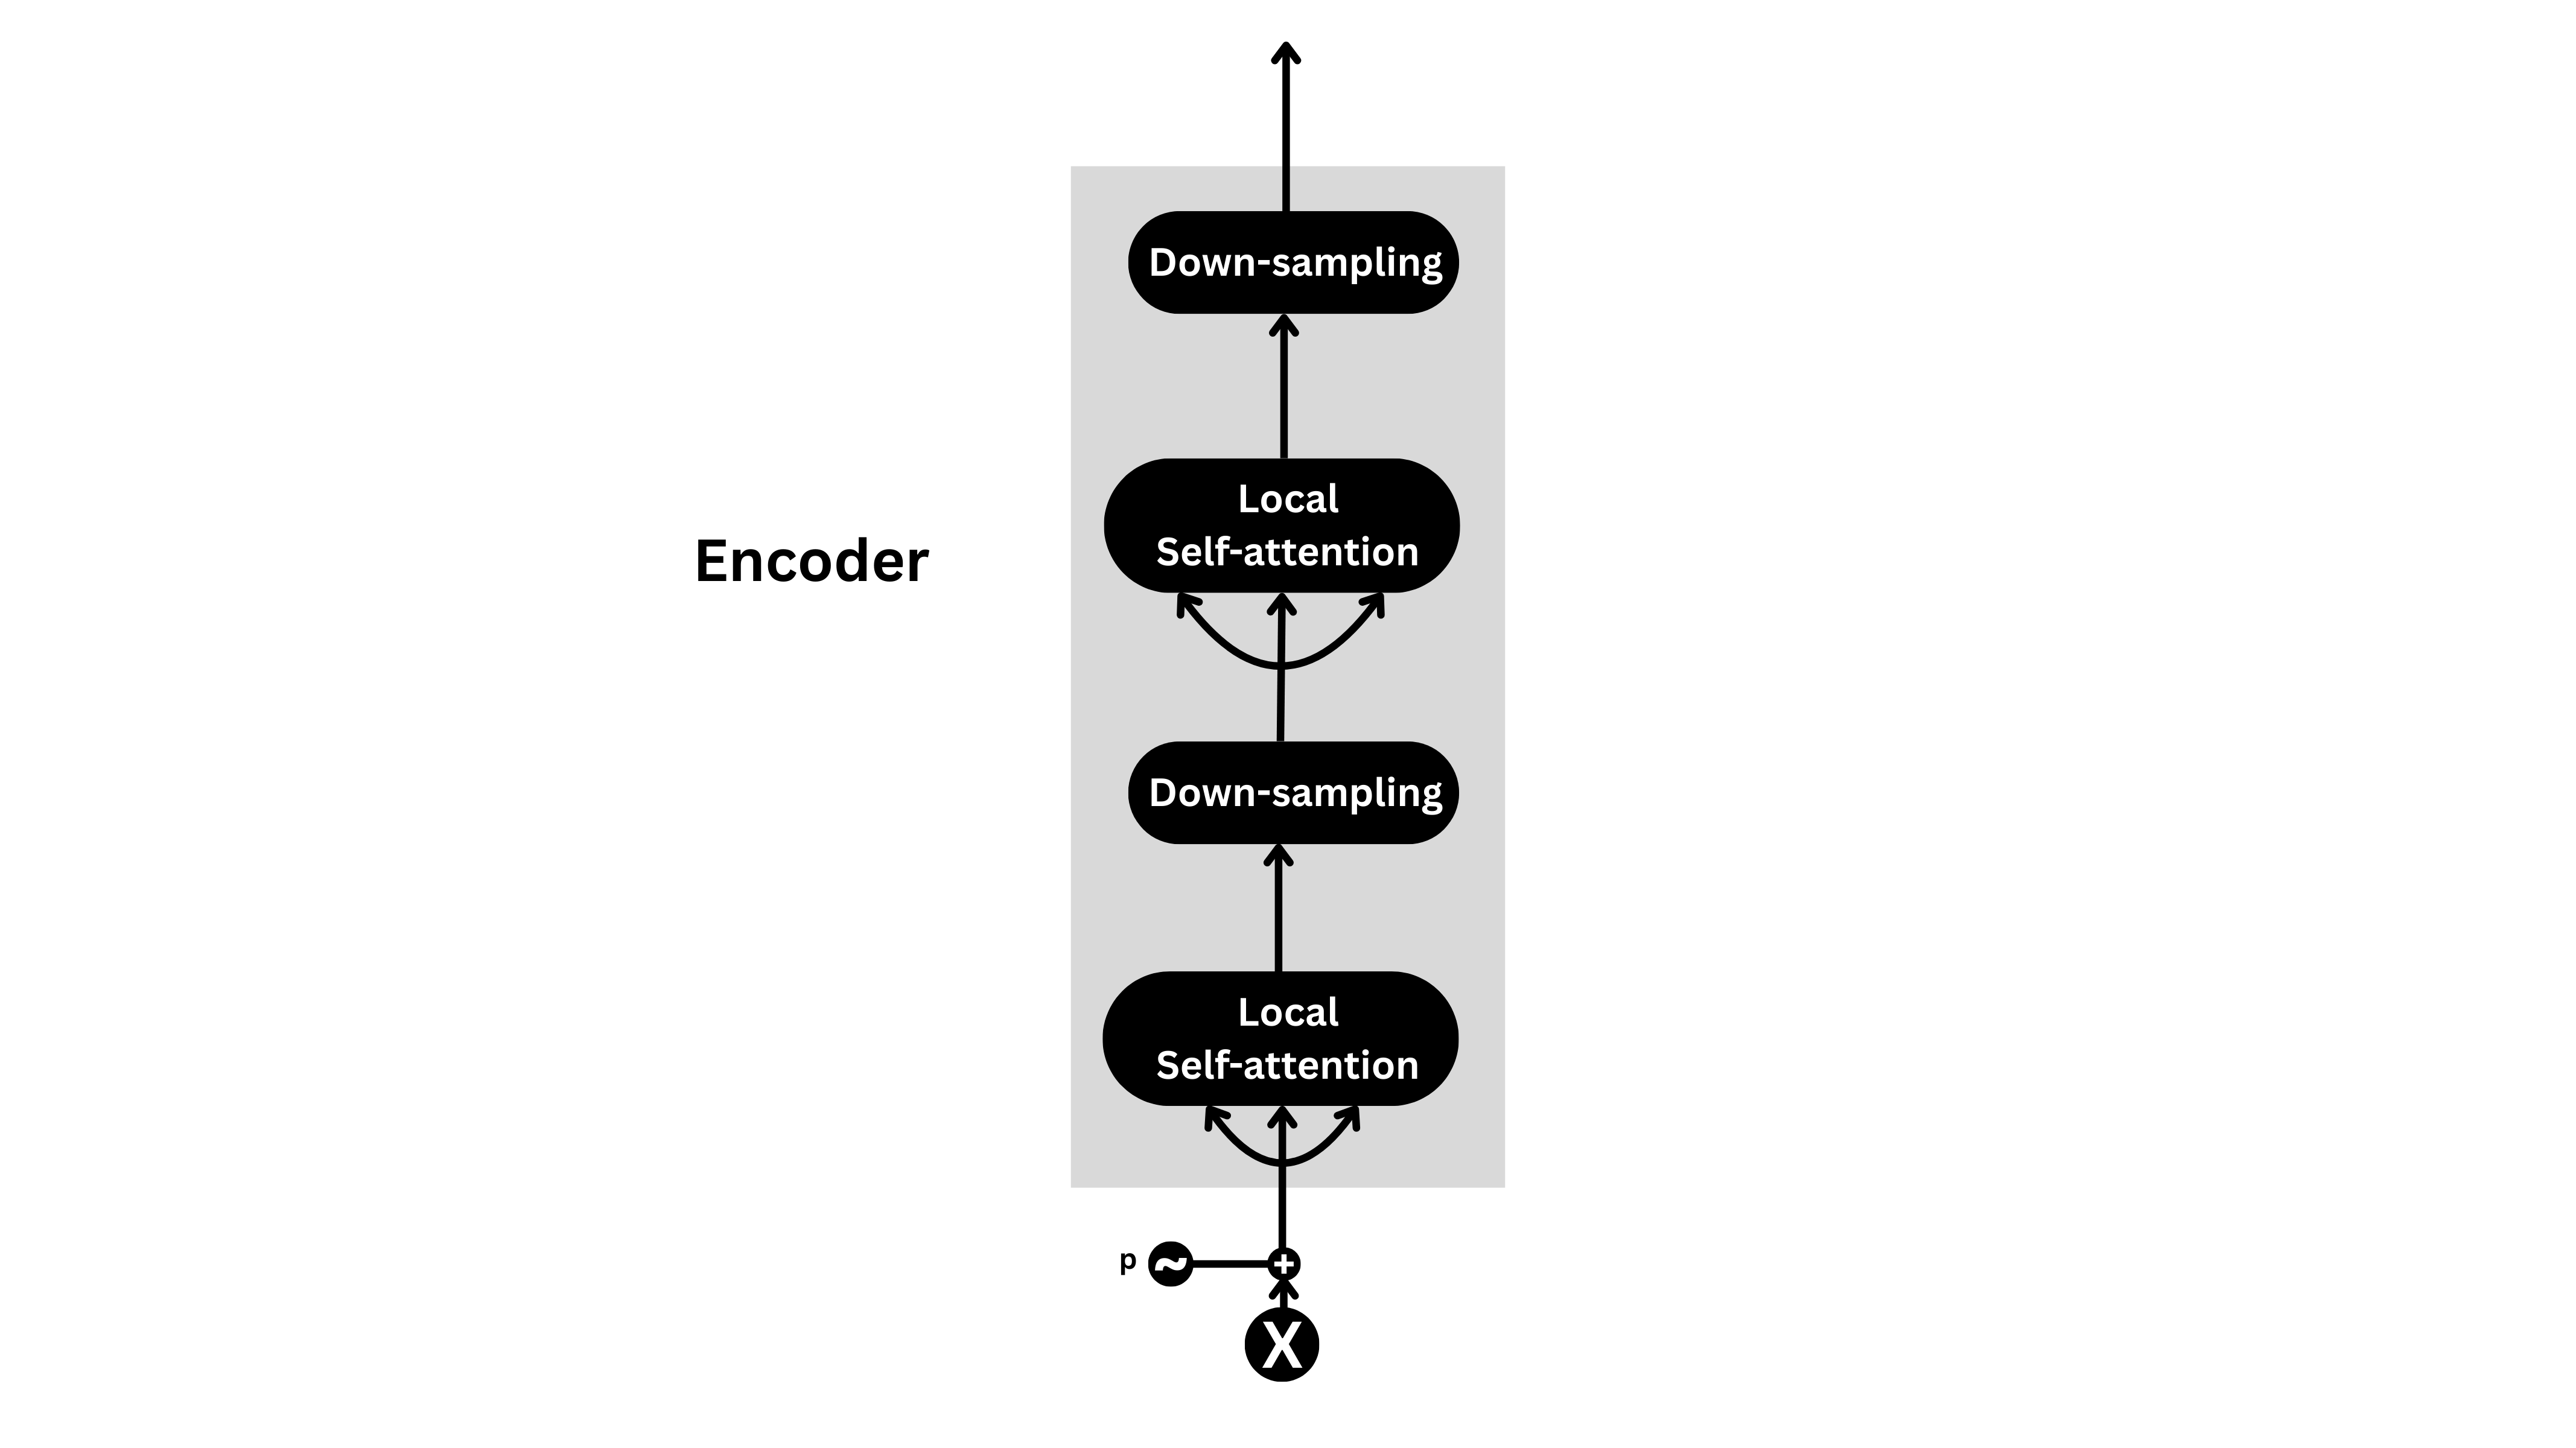
\includegraphics[width=1\textwidth]{images/Encoder.png}
\caption{\centering Encoder of nnFormer}
\label{Fig:encoder}
\end{figure}

Each of the \gls{lvmsa} blocks is further comprised of successive layers of transformer modules in order to use attention mechanisms to effectively model the very intricate local interactions contextually. The encoder also combines very strategically placed downsampling convolutional layers which reduces the spatial dimensions of the feature maps while at the same time progressively increasing the depth of the feature map. This downsampling process helps the extraction of the hierarchical features in a more abstract way and on a global scale based representations at lower resolutions, which are essential for capturing the broader variations and anatomical structures.

\subsection{Bottleneck}
In the center of the nnFormer there is a bottleneck ,shown in \cref{Fig:bottleneck}. This bottleneck has \gls{gvmsa} (\gls{gvmsa}) mechanisms. Contrary to the \gls{lvmsa}, the \gls{gvmsa} provides with a significantly bigger receptive field which captures the long-range dependencies across the whole global context of the volumetric feature map. This increased area of the receptive field is essential at this stage in order to allow the network to achieve a comprehensive understanding of the global representation and the anatomical structures, improving the overall segmentation accuracy. The bottleneck very effectively combines the complex spatial dependencies and also the high level features which are extracted by the encoder. This serves as a robust foundation for the decoder for accurate and consistent output during the decoding.

\begin{figure}[htb!] % Changed from figure* to figure unless you specifically need double-column
\centering
% \begin{subfigure}[b]{1.5\textwidth} 
\centering
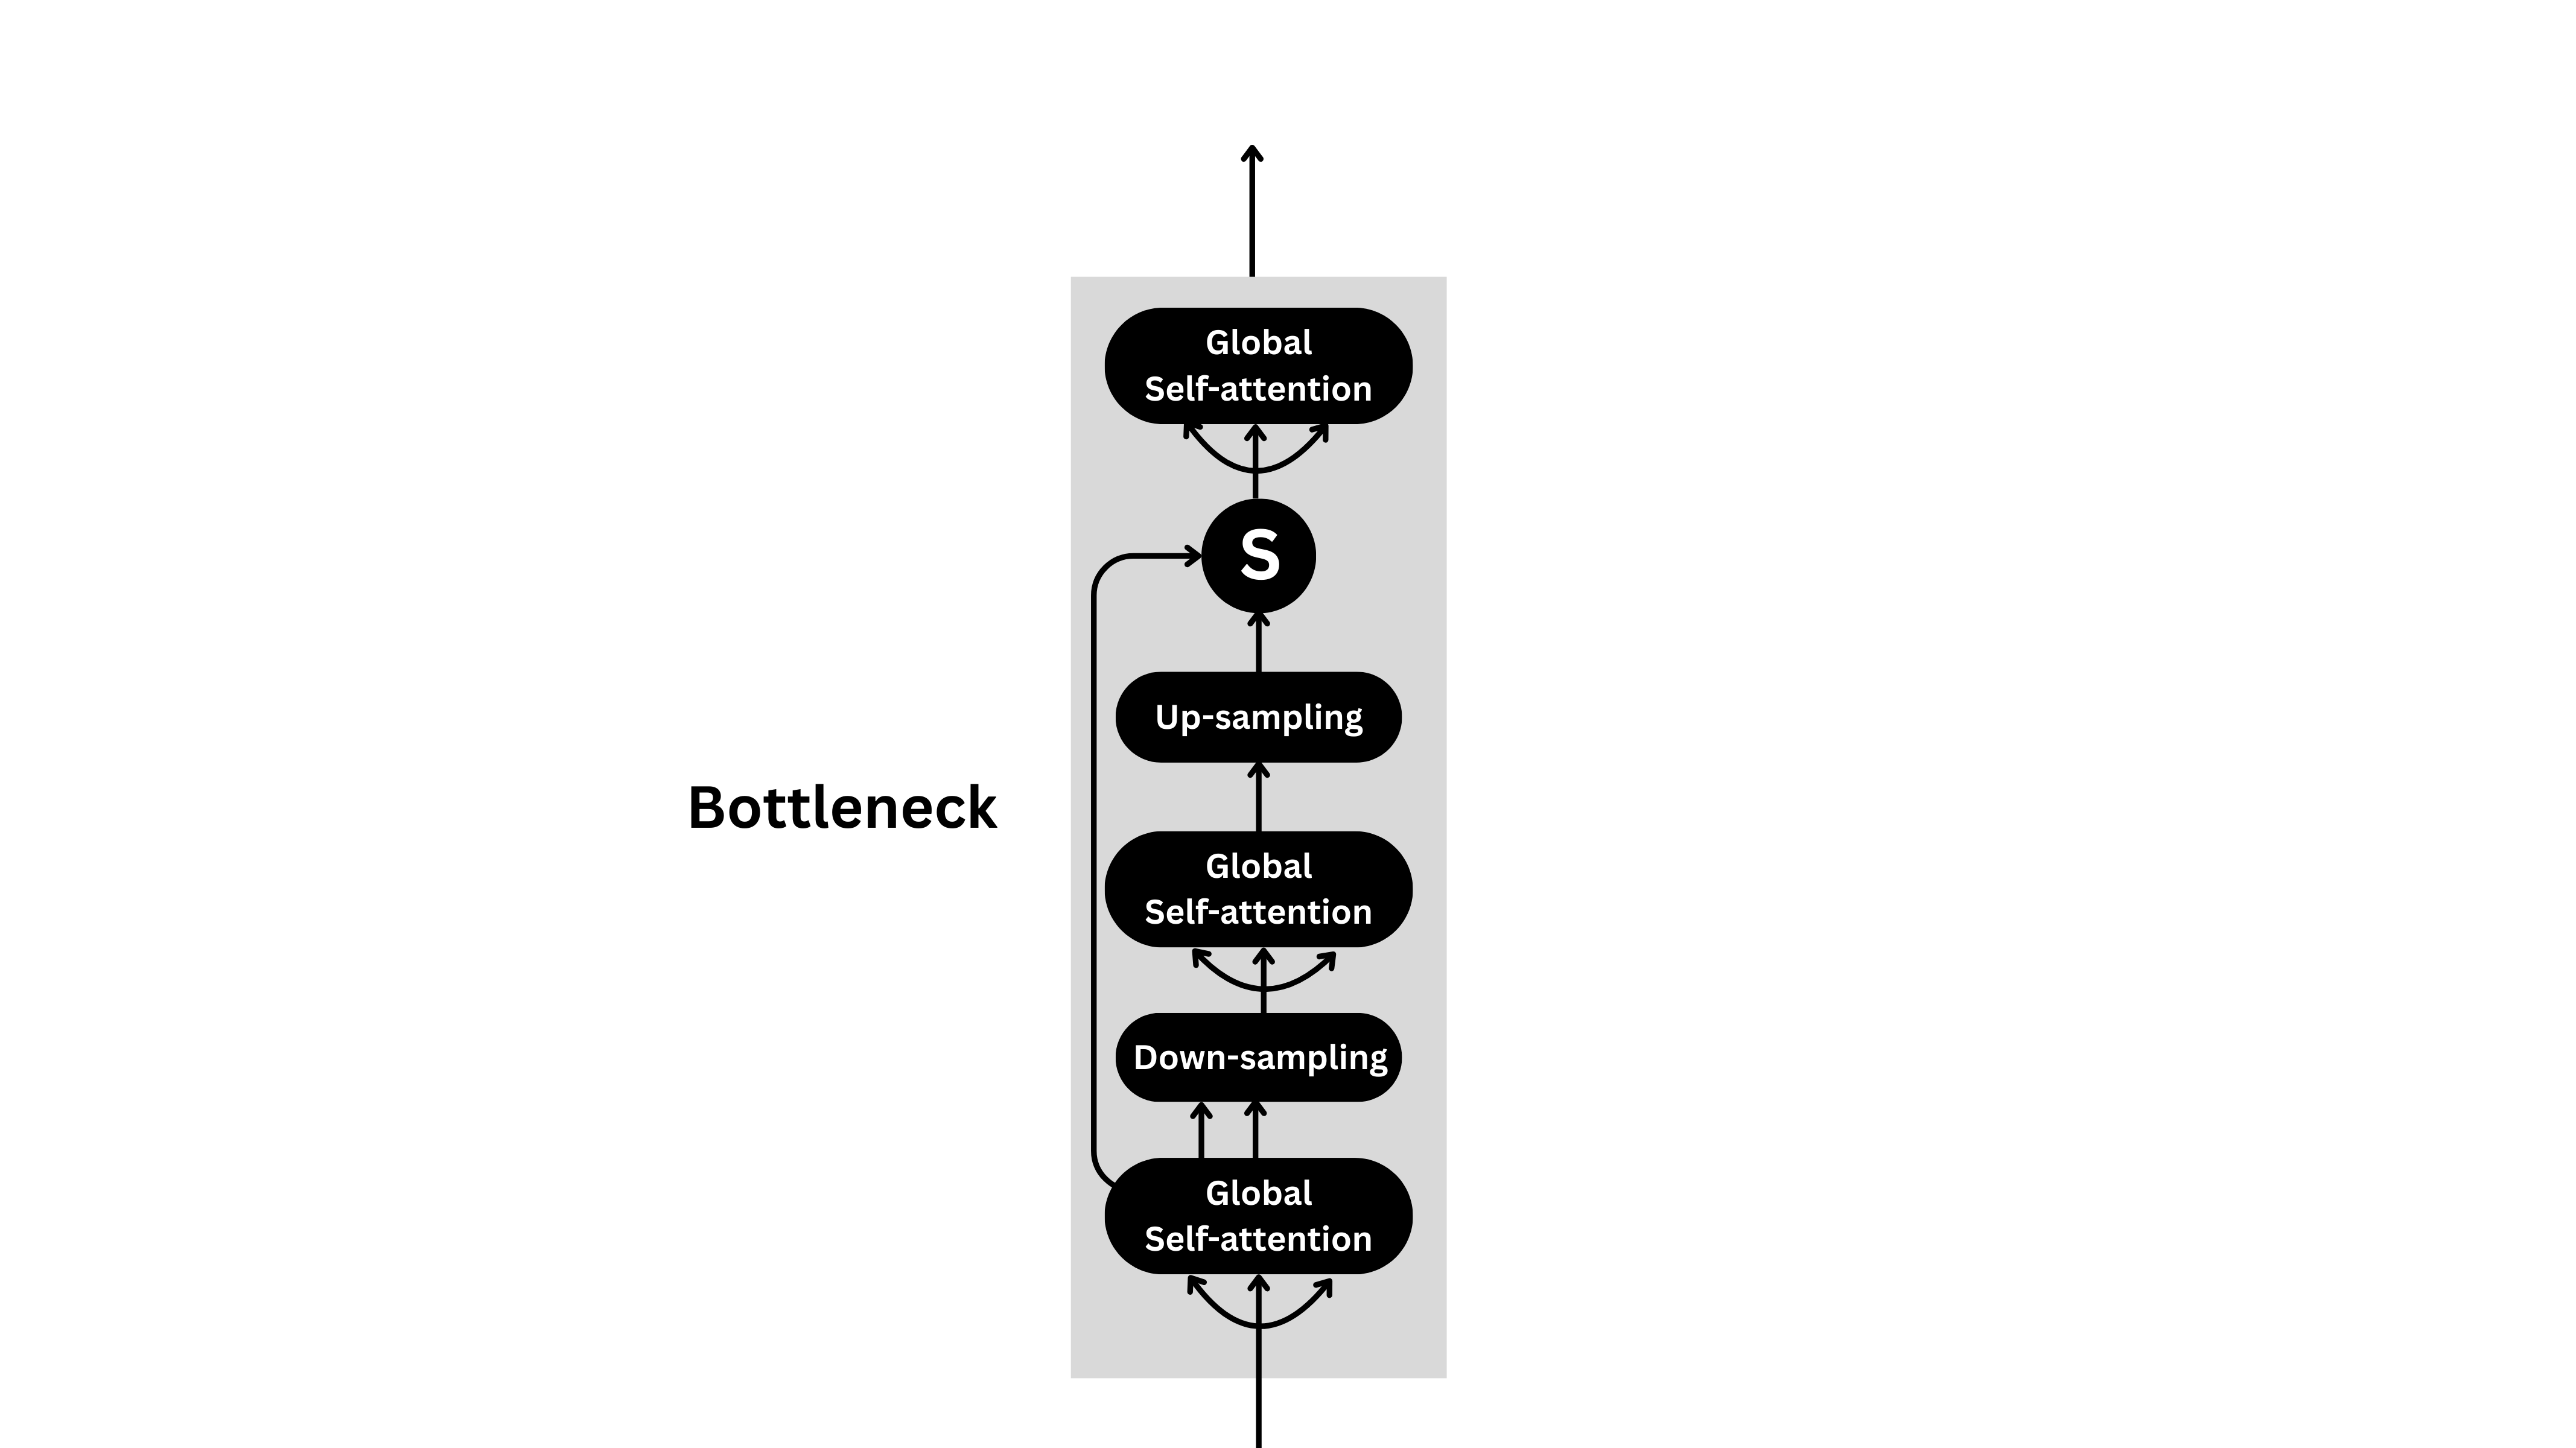
\includegraphics[width=1\textwidth]{images/Bottleneck.png}
\caption{\centering Bottleneck of nnFormer}
\label{Fig:bottleneck}
\end{figure}

\subsection{Decoder}
The decoder, in \cref{Fig:decoder} is, in a way, mirrored version of the encoder it also employs \gls{lv}-MSA blocks but coupled with convolutional upsampling, instead of the downsampling, or so-called transposed convolution. This restores the spatial resolution of the feature maps gradually to the original dimensions of the input. Each step of the upsampling process in the decoder is designed so as to reconstruct the detailed anatomical information by combining the high resolution detail captured spatially from the corresponding encoding stages via skip connections. 

\begin{figure}[htb!] % Changed from figure* to figure unless you specifically need double-column
\centering
% \begin{subfigure}[b]{1.5\textwidth} 
\centering
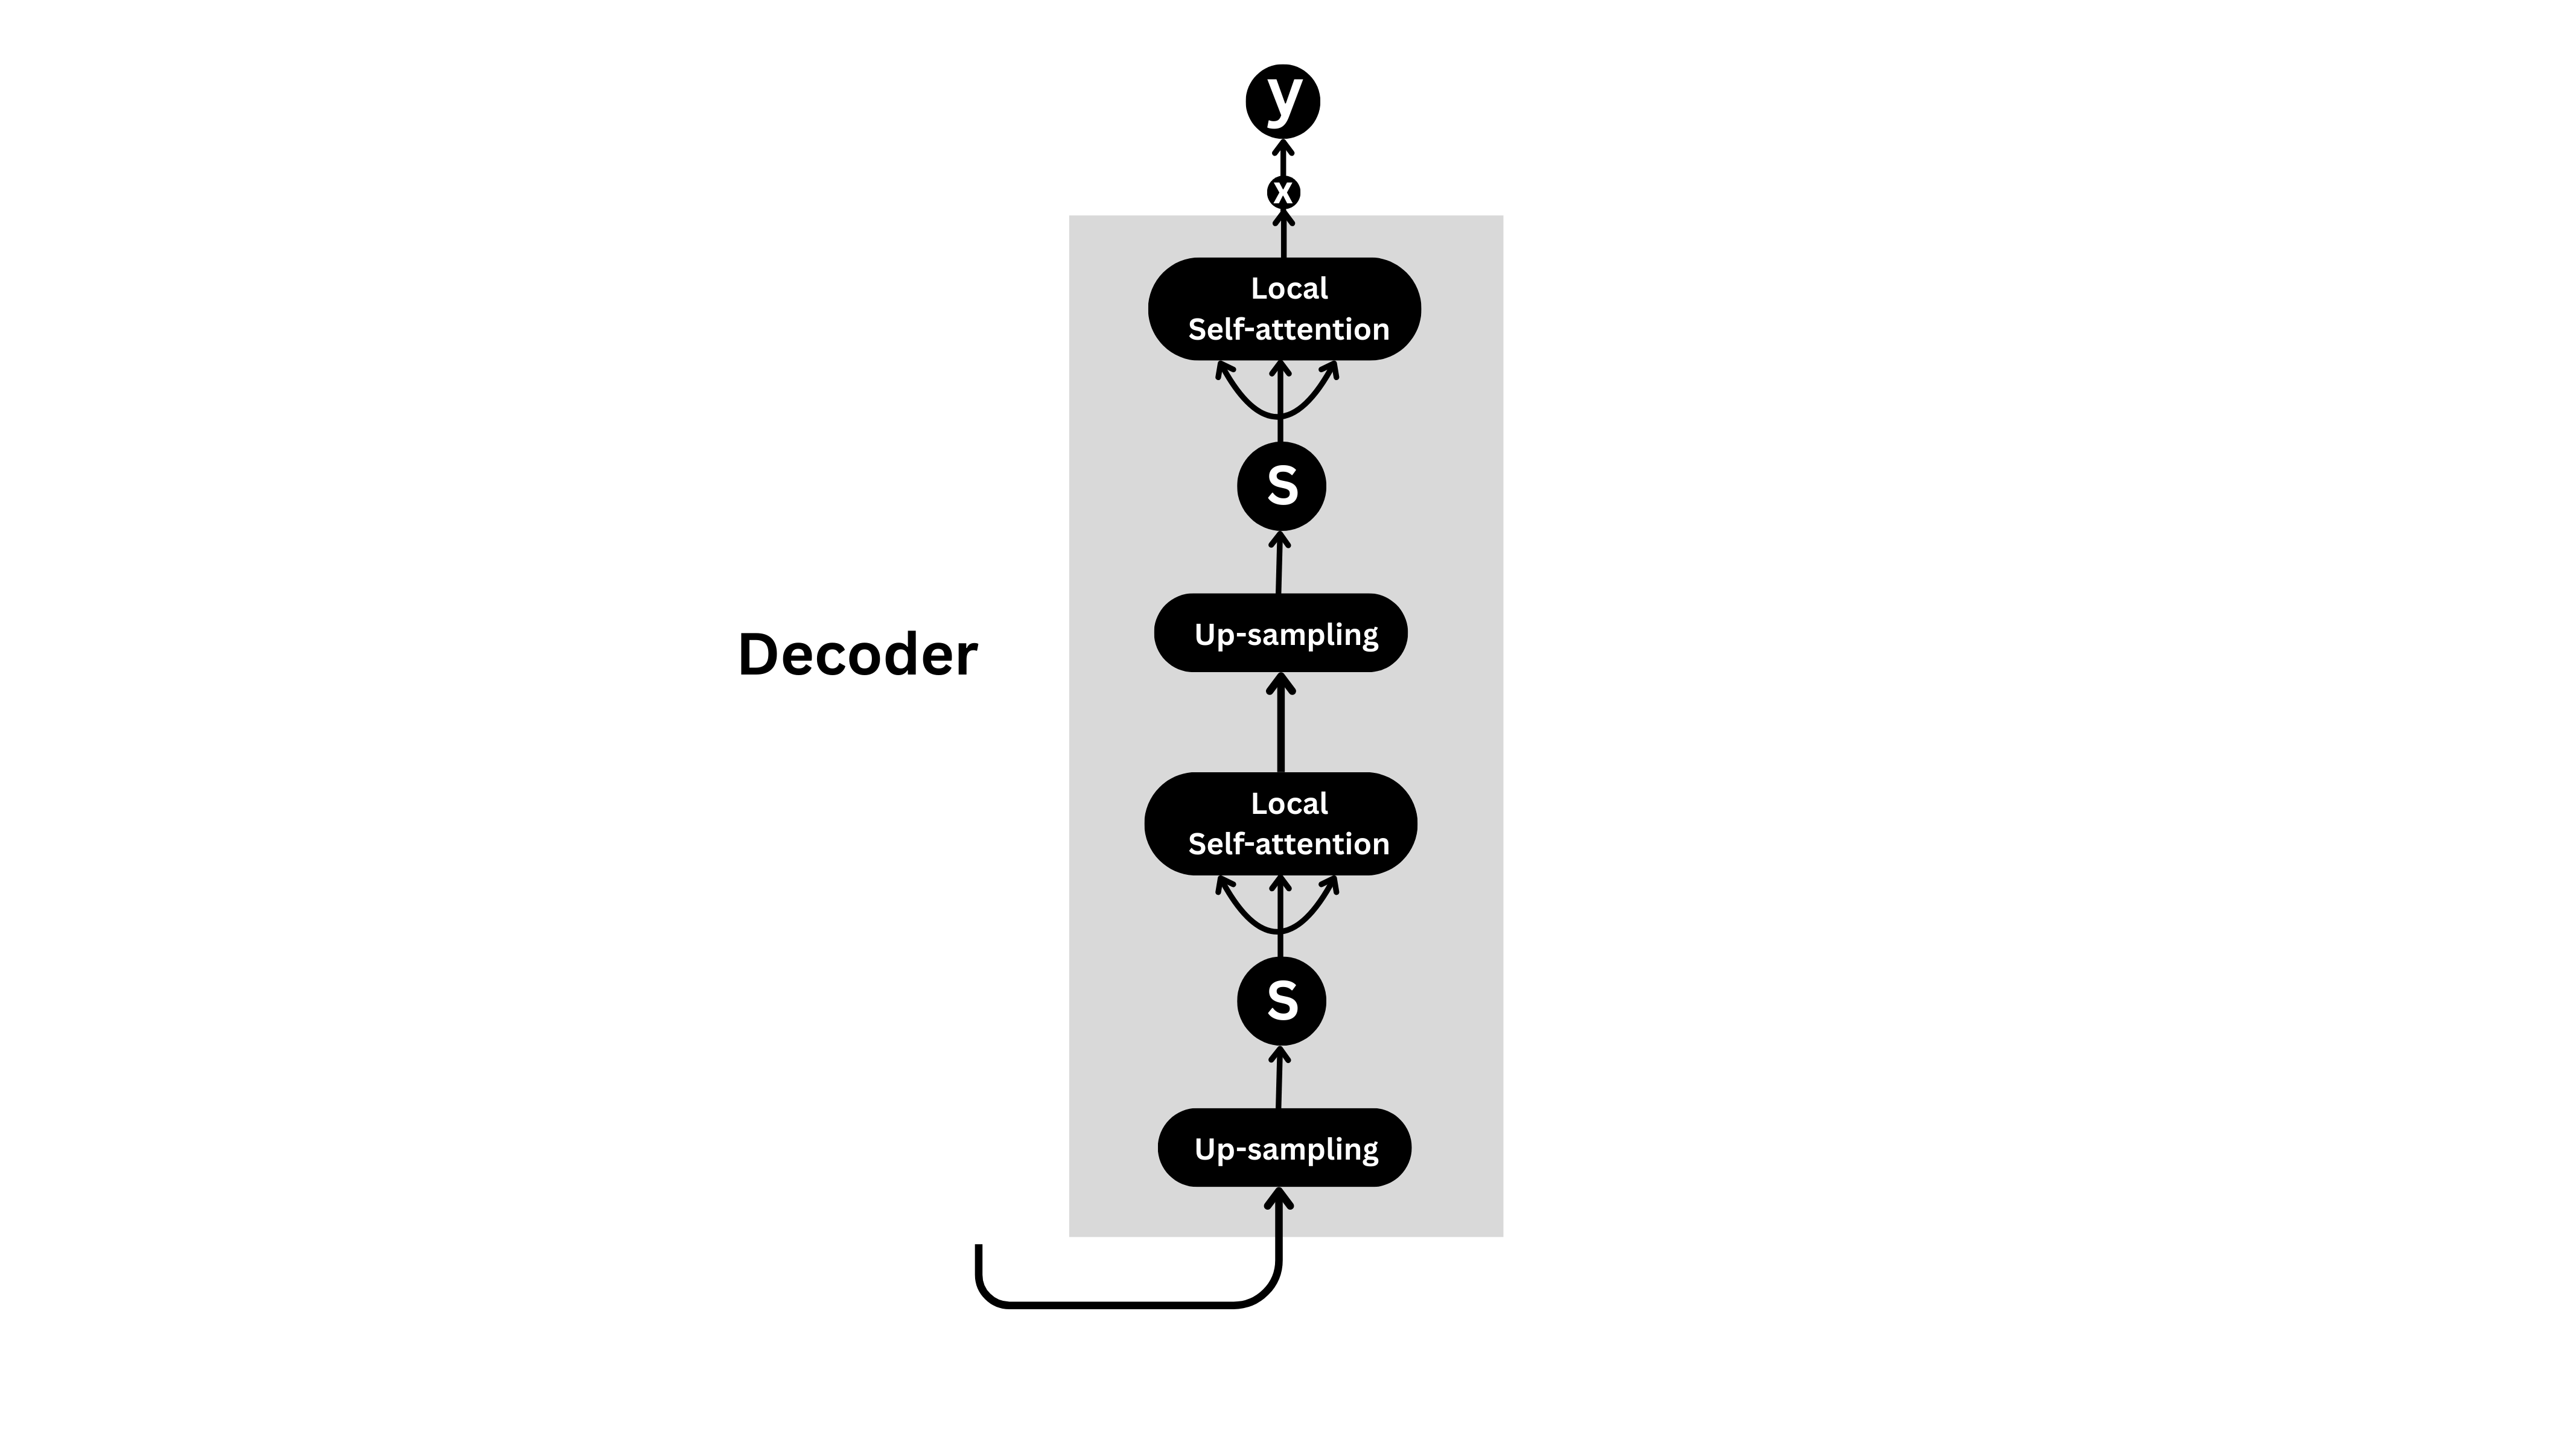
\includegraphics[width=1\textwidth]{images/Decoder.png}
\caption{\centering Decoder of nnFormer}
\label{Fig:decoder}
\end{figure}

A prime innovation of the nnFormer is the use of the skip attention mechanisms, in place of he traditional concatenation or summation which is typically used in skip connection mechanisms. These skip connections very selectively integrates the features of the encoder with the corresponding features of the decoder, which are guided by the attention weights that highlight relevant spatial features dynamically and hence suppress the irrelevant features. This selective combination majorly improves the precision of the segmentation, specifically in the areas where the clear anatomical delineation is very challenging due to the noise and artifacts.

\subsection{Attention Mechanisms}
nnFormer utilizes two different types of attention mechanisms: the \gls{lvmsa} and \gls{gvmsa}. \gls{lvmsa} very efficiently models the local spatial dependencies by partitioning the feature maps into manageable patches of volumes, which reduces the computational complexity without sacrificing a lot of the performance of the attention mechanism. In contrast to this, \gls{gvmsa} models the global interactions spatially across the entire volumetric feature maps, which are essential for capturing the large scale anatomical structural integrity and the contextual relationships. Both of the attention mechanisms use multi-head configurations which enable parallel computations of attention across multiple representational subspaces. This multi-ha design greatly improves the capability of the network in order to concurrently capture very diverse spatial relationships and the interactions at multiple scales hence thereby improving the segmentation accuracy.

\subsection{Integration and Optimization}
The amalgamation of \gls{lvmsa}, \gls{gvmsa} and the convolutional operations in the nnFormer is very carefully optimized in order to leverage the strength of each of these methods. The convolutional layers provide the efficient encoding of the low level spatual features, while the \gls{lvmsa} and the \gls{gvmsa} collectively capture both the complex spatial contexts and the long-range dependencies which are crucial for the precise and robust segmentation, providing us with the overall nnFormer architecture shown in \cref{Fig:nnformer}. Optimization of the nnFormer involves a specialized loss function called the Dice cross entropy loss (DiceCELoss). This loss function objectivises a high segmentation accuracy while maintaining a reliable realistic plausibility, which effectively guides the learning process towards more generalizable models across diverse imaging conditions.

\begin{figure}[htb!] 
\centering
% \begin{subfigure}[b]{1.5\textwidth} 
\centering
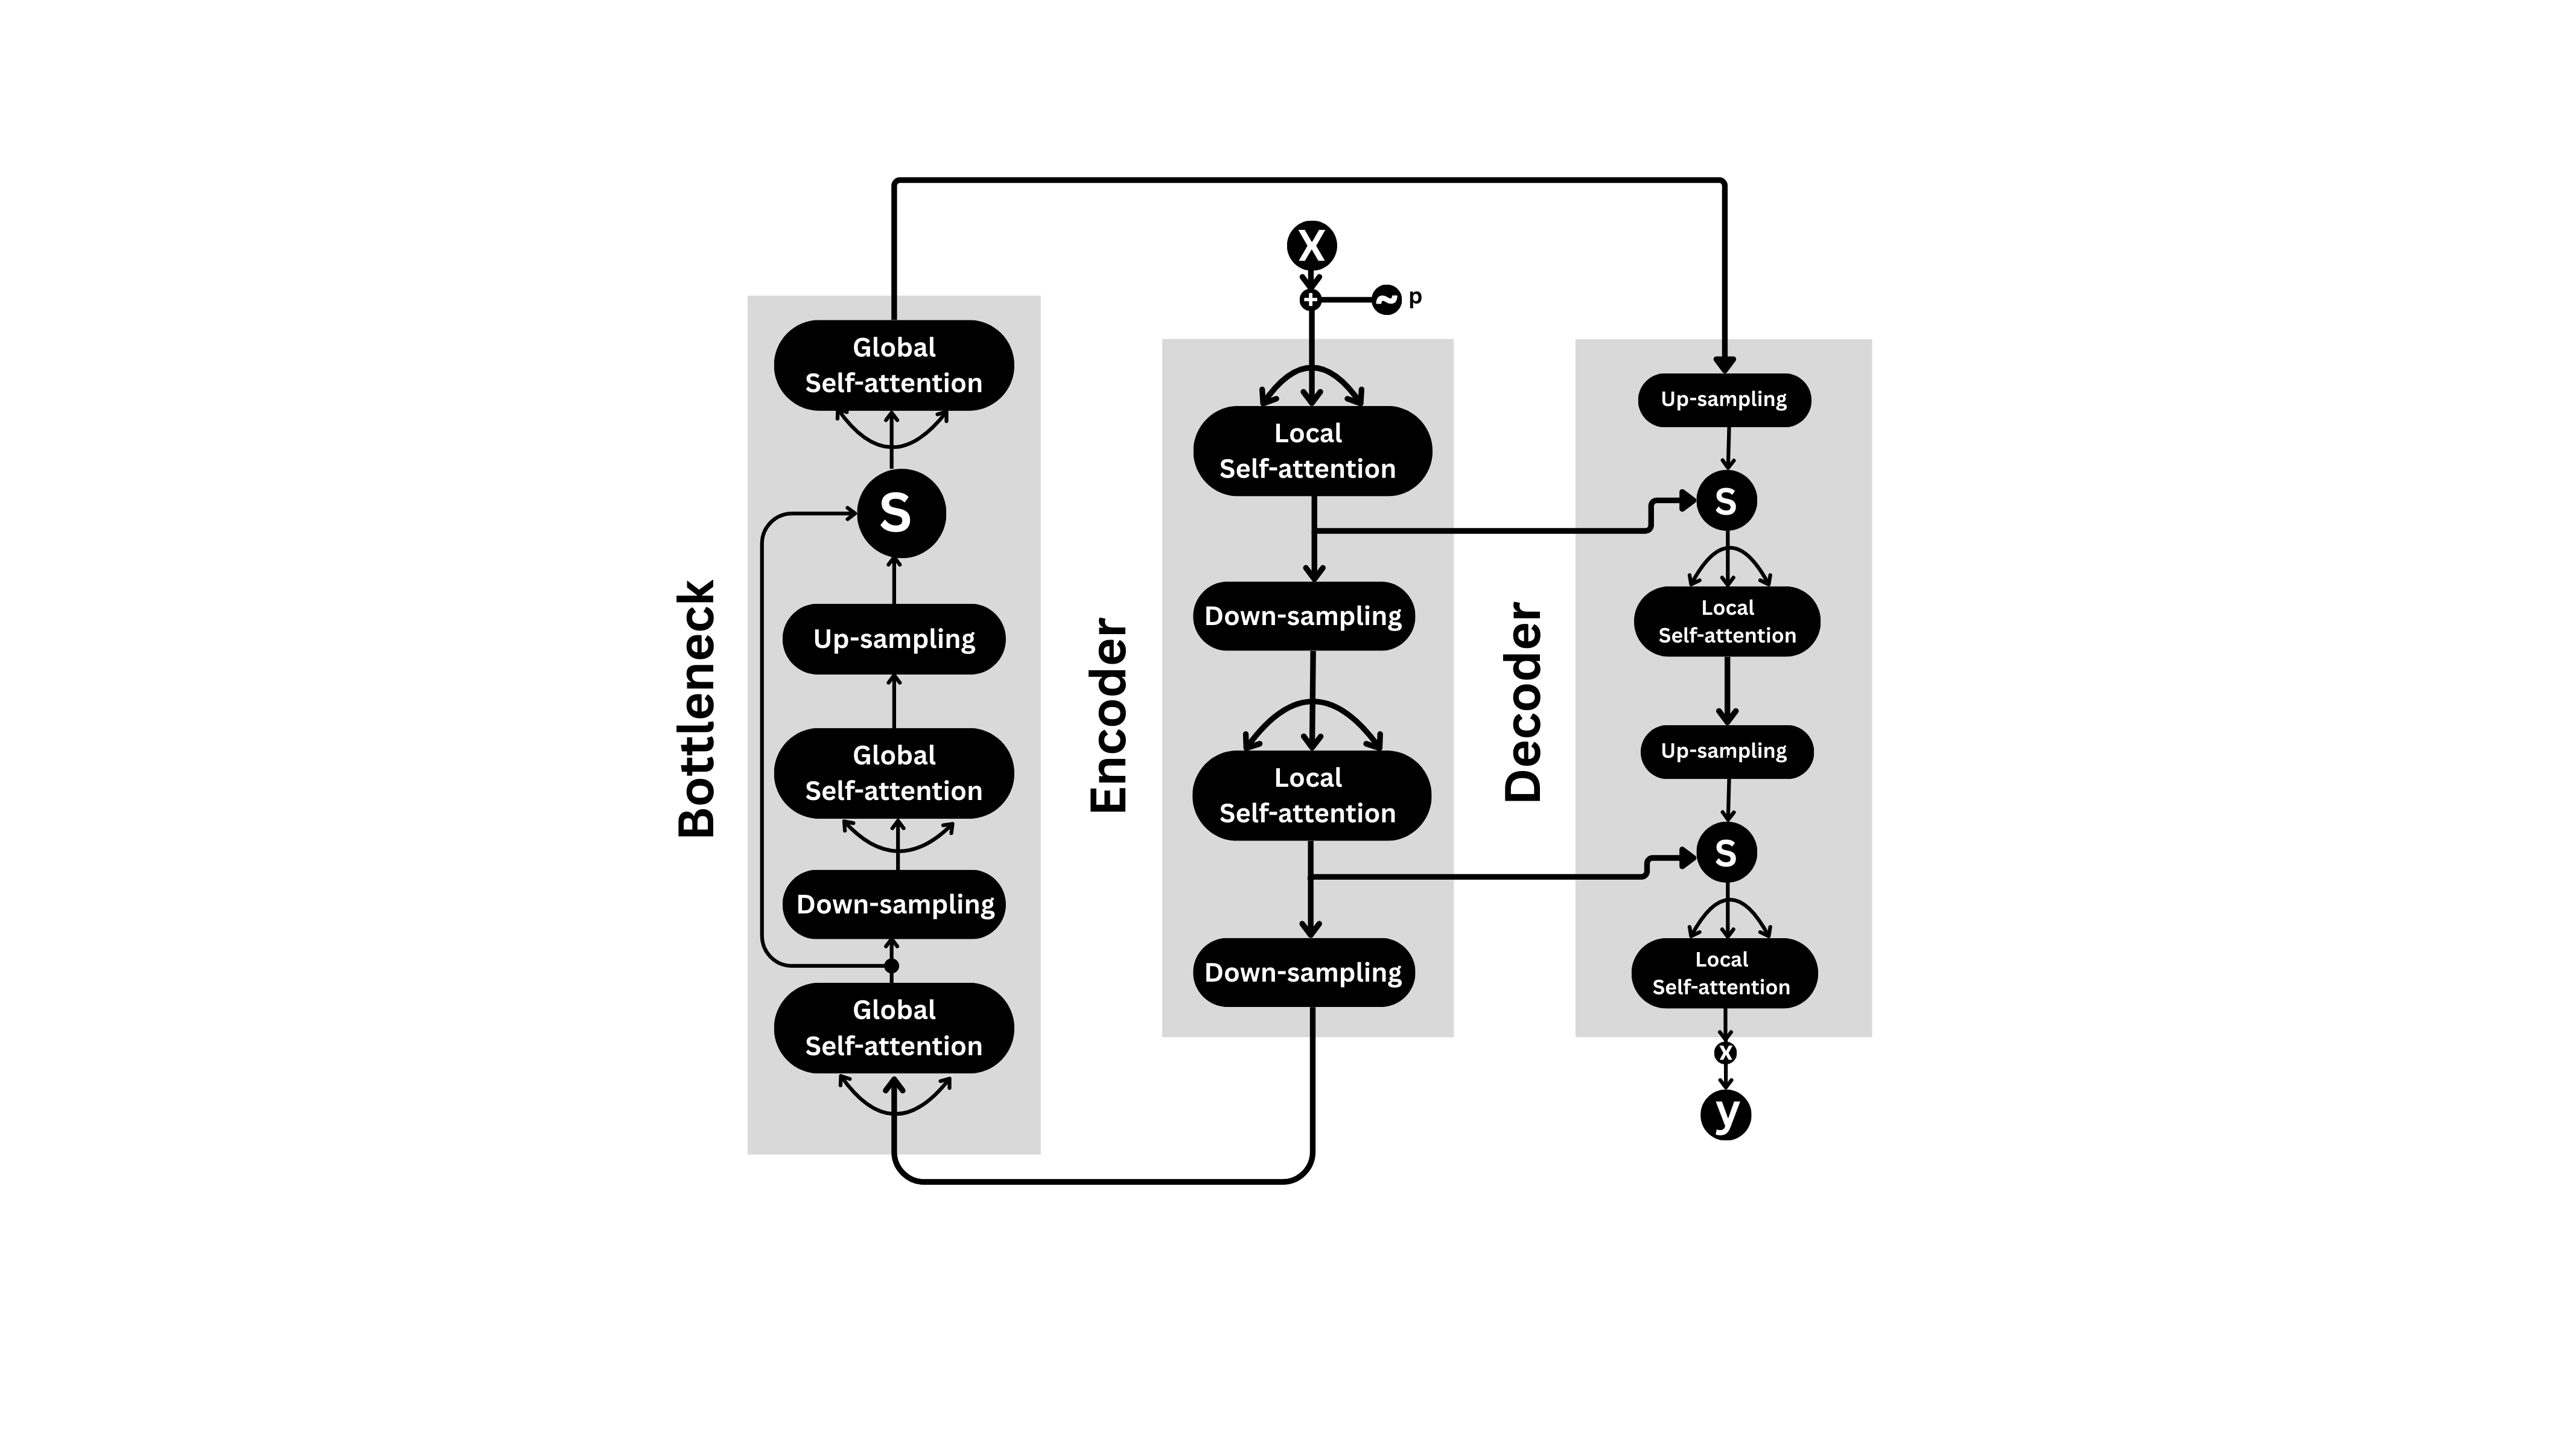
\includegraphics[width=1\textwidth]{images/Architecture.png}
\caption{\centering Full nnFormer architecture}
\label{Fig:nnformer}
\end{figure}

In conclusion, the nnFormer architecture represents a very sophisticated segmentation framework which is specifically tailored for medical imaging systems. The innovative design of the architecture and the advanced methods of attention overcomes the traditional limitations of segmentation models by effectively using optimization techniques across components ensuring accurate, robust and clinically meaningful segmentation outputs.

\section{Statistical Shape Prior}
\gls{ssp} offer a very powerful approach in order to enhance the robustness of the segmentation, specifically within the domain of medical imaging having data that might have sparse annotations available and noise embedded into it. In the context of \gls{mpi} \gls{spect}, SSPs are employed as a form of regularization technique that combined the prior knowledge about the left ventricular shape or its anatomy directly into the learning process of a \gls{dl} model. This section provides a comprehensive examination of the \gls{ssp} method which is used in this research including its theoretical, background, implementation and integration within the \gls{dl} pipeline.

\subsection{Motivation for SSPs}
Tradition \gls{dl} approaches often rely completely on the pixel-level intensities and their patterns in order to learn the segmentation boundaries. However, using this strategy can become very unreliable in low quality image settings, where the tissue boundaries are most of the time blurred or occluded due to the low resolution of images, noise in them, and partial volume effects. In order to address this issue, SSPs use a population level anatomical information in order to put a constraint on the segmentation process for plausible output shapes increasing the resilience to noise and variability. In \gls{mpi} \gls{spect}, the consistence delineation of the \gls{lv} is extremely critical for precise and accurate computation of the functional parameters of the cardiac imagery The shapes of the \gls{lv} vary across different patients but it maintains a stable topology that can be modeled statistically. SSPs capture this anatomical prior and provide a probabilistic framework that biases the training process towards valid segmentation outputs.

\subsection{Shape Prior Construction}
In order to contruct the shape priors, a mathematical model for the \gls{lv} is used which is used to generate a featr space. The input \gls{spect} volumes are first aligned to a common coordinate system using techniques such as affine or non-rigid registration. After the alignment, the shape representations are extracted, commonly as binary masks. In this work, the shapes are encoded using contoured vectors in a latent space that is suitable for probabilistic modeling. Once the shapes are aligned, Principal Component Analysis (PCA) is applied to the shape representations in order to identify the primary modes of variation. This gives out a low-dimensional shape space where each shape can actually be represented as a linear combination of the mean shape and a set of principal components. The statistical model can be expressed as:

\begin{equation} 
\addcontentsline{equ}{equations}{\protect\numberline{\theequation}Statistical Shape Model}
\text{S} = \bar{S} + \text{Pb}, 
\end{equation} 

where $\bar{S}$ is the mean shape, $P$ is the matrix of principal components, and $b$ is a vector of shape parameters.

The parameters $b$ follow a Gaussian distribution which is estimated from the volumes, which forms the basis of the shape prior and is used later to asses the possibility of a predicted shape.

\subsection{Regularization Using Mahalanobis Distance}
In order to integrate the \gls{ssp} into the learning, a shape regularization term is added to the loss. This term penalize the deviations from the learned shape space using Mahalanobis distance, which is defined as:

\begin{equation} 
\addcontentsline{equ}{equations}{\protect\numberline{\theequation}Mahalanobis Distance}
D_M(b) = (b - \mu)^T \Sigma^{-1} (b - \mu), 
\end{equation}

where $\mu$ and $\Sigma$ are the mean and covariance of the shape parameters from the training data.

The constraint forces the network to produce output shapes that lie in the distribution of the known shapes. It acts as a force that corrects and guides the model to produce good \gls{lv} geometries.

\subsection{KL Divergence-Based Optimization}
In addition to the Mahalanobis distance, a Kullback-Lieber (KL) divergence term is used in order to further align the predicted distribution of shapes with the prior one. The KL divergence quantifies the difference that exists between the predicted shape distribution $a(b)$ and the prior distribution $p(b)$:

\begin{equation} 
\addcontentsline{equ}{equations}{\protect\numberline{\theequation}KL Divergence}
D_{KL}(q || p) = \int q(b) \log \left(\frac{q(b)}{p(b)}\right) db. 
\end{equation}

This term is particularly useful when training any probabilistic model such as a variational autoencoder (VAE) in order to learn to generate a whole distribution of anatomical shapes.

\subsection{Integration into the Segmentation Network}
The integration of the \gls{ssp} into the segmentation network follows a specific architectural strategy, instead of applying the regularization on the standalone loss term, the key novelty lies in embedding the priors directly into the feature space of the network, which influences the decoder using enhanced intermediate representations. 

The process begins with sampling the shape prior from the learned statistical distribution which is conditioned on the features that are derived from the input volume of \gls{spect}. This priors reflects a anatomically likely structure that is aligned with the patient's scan, and selected from a low-dimensional latent shape space. For each of the sampled prior there are two metrics that are calculated The first is the Mahalanobis distance ($D_M$) and the second is the KL divergence ($D_{KL}$), which quantify how well the prior conforms with the expected shape. These metrics are then combined into a single scalar shape prior loss:

\begin{equation}
\addcontentsline{equ}{equations}{\protect\numberline{\theequation}Combined Shape Loss} 
\mathcal{L}{shape} = \lambda_1 D_M + \lambda_2 D{KL}, 
\end{equation}

where $\lambda_1$ and $\lambda_2$ are empirically tuned coefficients.

Instead of using this $\mathcal{L}_{shape}$ as a regularization term in the loss, first the derivative of this loss is calculated which gives a tensor providing the derivative on the surface of shape prior. This derivative is then reshaped into a tensor matching the spatial dimensions of the nnFormer bottleneck output. Then this reshaped loss derivative term is concatenated to with the bottleneck of the feature map. This results in a fused representation that encodes both the contextual features that are data driven and the shape information giving the anatomical constraints. The decoder then processes this combined tensor, enabling the final segmentation to benefit from the shape priors. This integration guides the feature propagation throughout the whole network, improving the spatial coherence and the consistency of the segmentation.

\section{Training and Optimization Procedures}
The training and optimization of the full segmentation framework were specifically designed to ensure the convergence and the generalization capability of the model across varying anatomies of the patients and different imaging conditions. The architecture was implemented using the PyTorch library and trained on high-performance Nvidia GPUs, leveraging both the nnFormer and the \gls{ssp} modules.

\subsection{Training Dataset and Splits}
The training dataset consisted on \gls{mpi} \gls{spect} scanes from 60 different patients These scans were carefully selected in order to ensure the variability in the type of the tracer used the quality of the image and the features of the anatomy. The validation/testing dataset consisted of 14 different scans from different patients. The stratification ensured proper and proportional representation of the collimator types and the demographics of the patients across split.

\subsection{Data Augmentation}
In order to improve the generalization capability and avoid over-fitting to the training data, several different data augmentation techniques were employed during the training phase. These include: 
\begin{itemize}
\item Random rotation \item Spatial padding (To ensure consistent input size) \item Random cropping 
\end{itemize}

All of the augmentation or transformations were applied in real time using the Monai library in order to maintain anatomical plausibility and preserving the label integrity.

\subsection{Loss Function}
The loss function that is used in the study is the DiceCELoss known as the Dice cross-entropy loss, which combines the functioning of both the dice coefficient and the cross entropy loss. This formulation focuses on 2 crucial aspects of the medical image segmentation, which are class imbalance and probabilistic boundary confidence.

The dice component of the loss function directly optimizes the function for the overlap the predicted labels and the ground truth which makes it very effective for the datasets that target the structures that occupy a small portion of the volume, which is what exists in myocardial \gls{spect}. Meanwhile the cross-entropy term ensures that the voxel-wise confidence of the classification is properly incorporated, allowing the whole network to learn the fine-grained details and maintain the sharp boundaries needed.

This hybrid loss is proved to be both differentiable and computaitonally efficient, with facilitates stable convergence during the training process. This loss was selected over te traditional single term losses due to the fact that its robustness in handling small, complex anatomical data even in the presence of noise. By relying completely on the the DiceCELoss, the training pipeline remains completely streamlined and very effective, which eliminates the need for additional tuning of the hyperparameters that is associated with the multi-loss formulations.

\begin{equation}
\text{DiceCELoss} = \left( 1 - \frac{2 \sum_{i} p_i g_i}{\sum_{i} p_i + \sum_{i} g_i} \right) - \sum_{i} g_i \log(p_i)
\end{equation}

In the above formulation, \( p_i \) represents the predicted probability for voxel \( i \), while \( g_i \) denotes the corresponding ground truth label, which is typically binary. The index \( i \) runs over all voxels (or pixels) in the image or volume. In the case of multi-class segmentation, the formulation extends to include an additional class index \( c \), where \( p_{i,c} \) indicates the predicted probability that voxel \( i \) belongs to class \( c \), and \( g_{i,c} \) is the one-hot encoded ground truth label for voxel \( i \) with respect to class \( c \). The terms \( \sum_i p_i \) and \( \sum_i g_i \) represent the total predicted and ground truth positive volumes, respectively, while \( \sum_i p_i g_i \) measures the overlap between prediction and ground truth. The cross-entropy component, \( \sum_i g_i \log(p_i) \), quantifies the voxel-wise classification error by penalizing deviations between predicted probabilities and ground truth labels. Together, the Dice coefficient term and the Cross-Entropy loss term jointly capture both region-level overlap and voxel-level classification confidence, promoting accurate and stable segmentation outputs.

\subsection{Optimization Strategy}
Model training used the Adam optimizer \cite{Kingma2015Adam} with the following configuration:

\begin{itemize} \item Initial learning rate: $1 \times 10^{-5}$ \item Learning rate decay: exponential decay with a factor of 0.01 every 10 epochs \item Batch size: 2 volumes per iteration \item Weight decay: $1 \times 10^{-6}$ \item Number of epochs: 100 for nnFormer baseline, 50 for proposed \gls{ssp}-integrated model \end{itemize}

The best performing model, based on the validation loss, is saved for final testing.

\subsection{Evaluation Pipeline}
Following the training, model performance was evaluated on the test set. For each volume of the patient, the output of the segmentation is generated in a single forward pass The predictions were post-processed using the morphological operations in order to remove isolated false positives and maintain region continuity. Quantitative metrics such as Dice coefficient, recall, precision, and F1 score were computed.

\subsection{Implementation Environment}
All of the training and evaluation procedures were conducted in a Linux based environment with CUDA-enabled GPUs. the full code was implemented in Python using PyTorch, with additional support of libraries such as monai, pandas, numpy and matplotlib fro visualisation. The rigorous training and the optimization pipeline ensured the resulting model was both the accurate and very generalizable which is robust against the variability of imaging, and is efficient enough for potential deployment in clinical settings.

\section{Implementation Details and Computational Environment}

In order to ensure the reproducibility,, optimal training efficiency and the scalability the whole segmentation framework was implemented using an extremely module \gls{dl} environment. This section details the stack of the software, the computational infrastructure and the engineering strategies which are adopted in order to support the development and the training, validation and testing phase.

\subsection{Software Framework}
The model is developed using Python, leveraging the \gls{dl} library PyTorch 1.12 version, due to its flexibility and the wide adoption of the library in the research community all across the computer science community. Other key supporting libraries used in the research are:

\begin{itemize} \item \textbf{Monai} for data loading, augmentation, and patch-based processing. \item \textbf{NumPy} for numerical operations. \item \textbf{Scikit-learn} for evaluation metrics and other machine learning tasks. \item \textbf{Matplotlib and Seaborn} for visualization of training curves and result analysis. \item \textbf{Pydicom and Nrrd} for medical image I/O, including support for DICOM and nrrd formats. \end{itemize}

\subsection{Hardware Infrastructure}
The training of the model was performed on a server which is equipped with NVIDIA GTX 1080Ti GPU. These resources enabled efficient handling of very large scale volumetric datasets and helped with Simultaneous experimentation. The training sessions were accelerated using:

\begin{itemize} \item CUDA 12.8 for GPU-accelerated matrix operations. \item cuDNN to optimize the neural network routines. \item PyTorch's automatic mixed precision (AMP) in order to reduce the usage of memories but without sacrificing the accuracy of the model. \end{itemize}

\section{Evaluation Metrics and Experimental Setup}
In order to correctly evaluate the performance of the proposed methodology for segmentation ,a very comprehensive set of quantitative metrics is utilized, together with a carefully structured experimental setup. These selected metrics were chosen in order to capture both the geometric consistency of the segmentation and also the anatomical plausibility across different imaging conditions.

\subsection{Evaluation Metrics}
The evaluation of the segmentation performance focused on the following key performance metrics:

\begin{itemize}
\item \textbf{Dice Similarity Coefficient (DSC):} Measures the overlap between the predicted and ground truth segmentations, defined as:
\begin{equation}
\addcontentsline{equ}{equations}{\protect\numberline{\theequation}Dice Coefficient}
\text{DSC} = \frac{2|P \cap G|}{|P| + |G|},
\end{equation}
where $P$ and $G$ denote the predicted and ground truth segmentations, respectively.
\item \textbf{Intersection over Union (IoU):} Provides an alternative measure of overlap, calculated as:
\begin{equation}
\addcontentsline{equ}{equations}{\protect\numberline{\theequation}Intersection over Union (IoU)}
\text{IoU} = \frac{|P \cap G|}{|P \cup G|},
\end{equation}
which balances sensitivity and specificity by considering both false positives and false negatives.
\item \textbf{Precision:} Indicates the proportion of predicted positive voxels that are truly positive, defined as:
\begin{equation}
\addcontentsline{equ}{equations}{\protect\numberline{\theequation}Precision}
\text{Precision} = \frac{TP}{TP + FP},
\end{equation}
where $TP$ is the number of true positives and $FP$ is the number of false positives. High precision implies fewer false positive segmentations.
\item \textbf{Recall (Sensitivity):} Measures the ability of the model to correctly identify all relevant voxels belonging to the target structure, given by:
\begin{equation}
\addcontentsline{equ}{equations}{\protect\numberline{\theequation}Recall}
\text{Recall} = \frac{TP}{TP + FN},
\end{equation}
where $FN$ is the number of false negatives. A high recall value indicates effective capture of the entire structure, even if some false positives occur.
\end{itemize}
These metrics were computed for all volumes in the test set and averaged to provide mean performance indicators, standard deviations, and confidence intervals.

\subsection{Experimental Protocols}

The multiple experiment-based configurations were employed in order to analyze the robustness and the generalizability of the proposed architecture:

\begin{enumerate}
\item \textbf{Baseline Comparison:} The base nnFormer architecture was trained and evaluated independently to establish a performance baseline.
\item \textbf{Shape Prior Augmentation:} The proposed integrated model combining nnFormer with \gls{ssp} was evaluated to quantify the impact of incorporating anatomical priors into the segmentation pipeline.
\item \textbf{Comparison with SwinUNETR:} The SwinUNETR model, using the same preprocessing and hyperparameter configurations as nnFormer, was trained and evaluated to provide a comparative benchmark.
\item \textbf{Noise Robustness Analysis Using Shape Priors:} Robustness to image degradation was tested by introducing Poisson noise to phantom images generated from the shape prior model. These phantoms served as synthetic input \gls{spect} volumes, allowing evaluation of the model's ability to handle severely noisy conditions.

\item \textbf{Low Data Regime Simulation:} Subsampling experiments were conducted to evaluate segmentation performance under limited labeled data conditions (using 10, 20, 30 40 and 50 patients) and the performances for both the nnFormer and the nnFormer+\gls{ssp} were compared.

\end{enumerate}

These experimental evaluations comprehensively demonstrate the efficiency, the clinical reliability and the generalization capability of the nnFormer integrated with the \gls{ssp} model across a ranging \gls{mpi} \gls{spect} scenarios.

\section{Summary and Justification of Methodology}
The choices made about the methodology in this study were guided by the combined objectives of achieving \gls{sota} accuracy of segmentation and also ensuring the robustness of the method under constraints in a clinical setting, which include limited annotated data and high variance in the \gls{mpi} \gls{spect} image quality. Each component of the proposed architecture was selected specifically in order to address the challenges that are observed in the previous studies done in medical image segmentation approaches. The adoption of nnFormer as the backbone of the whole architecture is justified because of its ability to model global spatial dependencies and also the contextual relationships, which are most of the times very crucial for resolving ambiguities in a low resolution an high noise volumetric scans. Unlike the conventional \gls{cnn}-based architectures operating usually with limited receptive fields, structure of the nnFormer based on transformers allows the model to learn long-range anatomical correlations within the entire volume.

Despite the advantages offered by the transformer-based architectures such as the nnFormer they still require a large amount of data to learn effectively. In order to overcome this limitation and enhance the generalizability considering low data settings, the \gls{ssp} integration was introduced in the architecture. This update helps the model b embedding domain knowledge into the \gls{dl} model training phase as a way of providing anatomical regularization. This method provides a constraint to the segmentation model's output to plausible shapes, hence enhancing the reliability especially in cases that are challenging to work with suc as scans having perfusion defects or motion artifacts. The inclusion of this \gls{ssp} focuses on an important gap that exists in the existing methods. Traditional CNNs, and even transformer models can produce segmentation that might be structurally not plausibile, especially when faced with data that is noisy or sparse. By incorporating the shape regularization, which is based on the Mahalanobis distance and the KL divergence penalty, the proposed methodology ensures that the model adheres to expected anatomical configurations, but not at the cost of flexibility in the learning of the data. This balance is very critical in order to maintain credibility in real-world clinical applications.

In addition to all of this, the loss function, so-called the DiceCELoss, was motivated by the need of balancing the pixel-wise accuracy with the anatomical correctness of the output. This hybrid loss contributes to having consistency during the convergence process during the training phase, all the while promoting accuracy of the segmentation in both common and edge-case scenarios. Another very important decision was the use of multiple experimental protocols including the baseline comparisions of nnFormer and the SwinUNETR with our proposed architecture, and noise robust testing. All of these experiments were structured to validate the performance improvements and also to assess the generalizability of the model across multiple different imaging conditions. From the perspective of implementation, the usage of high-performance GPU hardware and a scalable software design ensured that the model is very efficiently trained and tested.


\cleardoublepage

\chapter{Developer documentation}
\label{ch:impl}

Lorem ipsum dolor sit amet, consectetur adipiscing elit. Duis nibh leo, dapibus in elementum nec, aliquet id sem. Suspendisse potenti. Nullam sit amet consectetur nibh. Donec scelerisque varius turpis at tincidunt.


\section{Theorem-like environments}

\begin{definition}
Mauris tristique sollicitudin ultrices. Etiam tristique quam sit amet metus dictum imperdiet. Nunc id lorem sed nisl pulvinar aliquet vitae quis arcu. Morbi iaculis eleifend porttitor.
\end{definition}

Maecenas rutrum eros sem, pharetra interdum nulla porttitor sit amet. In vitae viverra ante. Maecenas sit amet placerat orci, sed tincidunt velit. Vivamus mattis, enim vel suscipit elementum, quam odio venenatis elit, et mollis nulla nunc a risus. Praesent purus magna, tristique sed lacus sit amet, convallis malesuada magna. Phasellus faucibus varius purus, nec tristique enim porta vitae.

\begin{theorem}
Nulla finibus ante vel arcu tincidunt, ut consectetur ligula finibus. Mauris mollis lectus sed ipsum bibendum, ac ultrices erat dictum. Suspendisse faucibus euismod lacinia. Etiam vel odio ante.
\end{theorem}
\begin{proof}
Etiam pulvinar nibh quis massa auctor congue. Pellentesque quis odio vitae sapien molestie vestibulum sit amet et quam. Pellentesque vel dui eget enim hendrerit finibus at sit amet libero. Quisque sollicitudin ultrices enim, nec porta magna imperdiet vitae. Cras condimentum nunc dui.
\end{proof}

Donec dapibus sodales ante, at scelerisque nunc laoreet sit amet. Mauris porttitor tincidunt neque, vel ullamcorper neque pulvinar et. Integer eu lorem euismod, faucibus lectus sed, accumsan felis. 

\begin{remark}
Nunc ornare mi at augue vulputate, eu venenatis magna mollis. Nunc sed posuere dui, et varius nulla. Sed mollis nibh augue, eget scelerisque eros ornare nec. Praesent porta, metus eget eleifend consequat, eros ligula eleifend ex, a pellentesque mi est vitae urna. Vivamus turpis nunc, iaculis non leo eget, mattis vulputate tellus.
\end{remark}

Fusce in aliquet neque, in pretium sem. Donec tincidunt tellus id lectus pretium fringilla. Nunc faucibus, erat pretium tempus tempor, tortor mi fringilla neque, ac congue ex dui vitae mauris. Donec pretium et quam a cursus.

\begin{note}
Aliquam vehicula luctus mi a pretium. Nulla quam neque, maximus nec velit in, aliquam mollis tortor. Aliquam erat volutpat. Curabitur vitae laoreet turpis. Integer id diam ligula.
\end{note}

Ut sollicitudin tempus urna et mollis. Aliquam et aliquam turpis, sed fermentum mauris. Nulla eget ex diam. Donec eget tellus pharetra, semper neque eget, rutrum diam.

\subsection{Equations, formulas}

Duis suscipit ipsum nec urna blandit, $2 + 2 = 4$ pellentesque vehicula quam fringilla. Vivamus euismod, lectus sit amet euismod viverra, dolor metus consequat sapien, ut hendrerit nisl nulla id nisi. Nam in leo eu quam sollicitudin semper a quis velit.

$$a^2 + b^2 = c^2$$

Phasellus mollis, elit sed convallis feugiat, dolor quam dapibus nibh, suscipit consectetur lacus risus quis sem. Vivamus scelerisque porta odio, vitae euismod dolor accumsan ut.

In mathematica, identitatem Euleri (equation est scriptor vti etiam notum) sit aequalitatem Equation.:
\begin{equation}\label{eq:euler}
e^{i \times \pi} + 1 = 0
\end{equation}

Vestibulum ante ipsum primis in faucibus orci luctus et ultrices posuere cubilia curae; Nullam pulvinar purus at pharetra elementum.
Aequationes adsignans aequationis signum:
\begin{align}
	A & = \frac{\pi r^2}{2} \\
	& = \frac{1}{2} \pi r^2
\end{align}

Proin tempor risus a efficitur condimentum. Cras lobortis ligula non sollicitudin euismod. Fusce non pellentesque nibh, non elementum tellus.
Omissa numeratione aliquarum aequationum:
\begin{align}
	f(u) & =\sum_{j=1}^{n} x_jf(u_j) \nonumber \\
	& =\sum_{j=1}^{n} x_j \sum_{i=1}^{m} a_{ij}v_i \nonumber \\
	& =\sum_{j=1}^{n} \sum_{i=1}^{m} a_{ij}x_jv_i
\end{align}

\section{Source code samples}

Nulla sodales purus id mi consequat, eu venenatis odio pharetra. Cras a arcu quam. Suspendisse augue risus, pulvinar a turpis et, commodo aliquet turpis. Nulla aliquam scelerisque mi eget pharetra. Mauris sed posuere elit, ac lobortis metus. Proin lacinia sit amet diam sed auctor. Nam viverra orci id sapien sollicitudin, a aliquam lacus suscipit. Quisque ac tincidunt leo.

\lstset{caption={Hello World in C++}, label=src:cpp}
\begin{lstlisting}[language={C++}]
#include <stdio>

int main() 
{
	int c;
	std::cout << "Hello World!" << std::endl;

	std::cout << "Press any key to exit." << std::endl;
	std::cin >> c;
	
	return 0;
}
\end{lstlisting}

\lstset{caption={Hello World in C\#}, label=src:csharp}
\begin{lstlisting}[language={[Sharp]C}]
using System;
namespace HelloWorld
{
	class Hello 
	{
		static void Main() 
		{
			Console.WriteLine("Hello World!");
			
			Console.WriteLine("Press any key to exit.");
			Console.ReadKey();
		}
	}
}
\end{lstlisting}

\subsection{Algorithms}

A general Interval Branch and Bound algorithm is shown in Algorithm. An appropriate selection rule is applied in.
Source of example: \href{https://www.inf.u-szeged.hu/actacybernetica/}{Acta Cybernetica (this is a hyperlink)}.

\begin{algorithm}[H]
\caption{A general interval B\&B algorithm} 
\label{alg:ibb} 
\textbf{\underline{Funct}} IBB($S,f$)
\begin{algorithmic}[1] % display line numbers before every n line, here n = 1
\State Set the working list ${\cal L}_W$ := $\{S\}$ and the final list ${\cal L}_Q$ := $\{\}$     
\While{( ${\cal L}_W \neq \emptyset$ )} \label{alg:igoend}
	\State  Select an interval $X$ from ${\cal L}_W$ \label{step:selrule}\Comment{Selection rule}  
	\State Compute $lbf(X)$ \Comment{Bounding rule}		  
	\If{$X$ cannot be eliminated} \Comment{Elimination rule}
		\State Divide $X$ into $X^j,\ j=1,\dots, p$, subintervals   \Comment{Division rule}
		\For{$j=1,\ldots,p$}
			\If{$X^j$ satisfies the termination criterion} \Comment{Termination rule}
				\State Store $X^j$ in ${\cal L}_W$ 
			\Else
				\State Store $X^j$ in ${\cal L}_W$ 
			\EndIf
		\EndFor  
	\EndIf
\EndWhile
\State \textbf{return} ${\cal L}_Q$
\end{algorithmic}
\end{algorithm}

\cleardoublepage

\chapter{Conclusion}
\label{ch:sum}

Lorem ipsum dolor sit amet, consectetur adipiscing elit. In eu egestas mauris. Quisque nisl elit, varius in erat eu, dictum commodo lorem. Sed commodo libero et sem laoreet consectetur. Fusce ligula arcu, vestibulum et sodales vel, venenatis at velit. Aliquam erat volutpat. Proin condimentum accumsan velit id hendrerit. Cras egestas arcu quis felis placerat, ut sodales velit malesuada. Maecenas et turpis eu turpis placerat euismod. Maecenas a urna viverra, scelerisque nibh ut, malesuada ex.

Aliquam suscipit dignissim tempor. Praesent tortor libero, feugiat et tellus porttitor, malesuada eleifend felis. Orci varius natoque penatibus et magnis dis parturient montes, nascetur ridiculus mus. Nullam eleifend imperdiet lorem, sit amet imperdiet metus pellentesque vitae. Donec nec ligula urna. Aliquam bibendum tempor diam, sed lacinia eros dapibus id. Donec sed vehicula turpis. Aliquam hendrerit sed nulla vitae convallis. Etiam libero quam, pharetra ac est nec, sodales placerat augue. Praesent eu consequat purus.

\cleardoublepage

% Acknowledgements (optional) - in case your thesis received funding or would like to express special thanks to someone
\chapter*{\acklabel}
\addcontentsline{toc}{chapter}{\acklabel}
In case your thesis received financial support from a project or the university, it is usually required to indicate the proper attribution in the thesis itself. Special thanks can also be expressed towards teachers, fellow students and colleagues who helped you in the process of creating your thesis.

% Appendices (optional) - useful for detailed information in long tables, many and/or large figures, etc.
\appendix
\chapter{Simulation results}
\label{appx:simulation}

Lorem ipsum dolor sit amet, consectetur adipiscing elit. Pellentesque facilisis in nibh auctor molestie. Donec porta tortor mauris. Cras in lacus in purus ultricies blandit. Proin dolor erat, pulvinar posuere orci ac, eleifend ultrices libero. Donec elementum et elit a ullamcorper. Nunc tincidunt, lorem et consectetur tincidunt, ante sapien scelerisque neque, eu bibendum felis augue non est. Maecenas nibh arcu, ultrices et libero id, egestas tempus mauris. Etiam iaculis dui nec augue venenatis, fermentum posuere justo congue. Nullam sit amet porttitor sem, at porttitor augue. Proin bibendum justo at ornare efficitur. Donec tempor turpis ligula, vitae viverra felis finibus eu. Curabitur sed libero ac urna condimentum gravida. Donec tincidunt neque sit amet neque luctus auctor vel eget tortor. Integer dignissim, urna ut lobortis volutpat, justo nunc convallis diam, sit amet vulputate erat eros eu velit. Mauris porttitor dictum ante, commodo facilisis ex suscipit sed.

Sed egestas dapibus nisl, vitae fringilla justo. Donec eget condimentum lectus, molestie mattis nunc. Nulla ac faucibus dui. Nullam a congue erat. Ut accumsan sed sapien quis porttitor. Ut pellentesque, est ac posuere pulvinar, tortor mauris fermentum nulla, sit amet fringilla sapien sapien quis velit. Integer accumsan placerat lorem, eu aliquam urna consectetur eget. In ligula orci, dignissim sed consequat ac, porta at metus. Phasellus ipsum tellus, molestie ut lacus tempus, rutrum convallis elit. Suspendisse arcu orci, luctus vitae ultricies quis, bibendum sed elit. Vivamus at sem maximus leo placerat gravida semper vel mi. Etiam hendrerit sed massa ut lacinia. Morbi varius libero odio, sit amet auctor nunc interdum sit amet.

Aenean non mauris accumsan, rutrum nisi non, porttitor enim. Maecenas vel tortor ex. Proin vulputate tellus luctus egestas fermentum. In nec lobortis risus, sit amet tincidunt purus. Nam id turpis venenatis, vehicula nisl sed, ultricies nibh. Suspendisse in libero nec nisi tempor vestibulum. Integer eu dui congue enim venenatis lobortis. Donec sed elementum nunc. Nulla facilisi. Maecenas cursus id lorem et finibus. Sed fermentum molestie erat, nec tempor lorem facilisis cursus. In vel nulla id orci fringilla facilisis. Cras non bibendum odio, ac vestibulum ex. Donec turpis urna, tincidunt ut mi eu, finibus facilisis lorem. Praesent posuere nisl nec dui accumsan, sed interdum odio malesuada.
\cleardoublepage

% Bibliography (mandatory)
\phantomsection
\addcontentsline{toc}{chapter}{\biblabel}
\printbibliography[title=\biblabel]
\cleardoublepage

% List of figures (optional) - useful over 3-5 figures
\phantomsection
\addcontentsline{toc}{chapter}{\lstfigurelabel}
\listoffigures
\cleardoublepage

% List of tables (optional) - useful over 3-5 tables
\phantomsection
\addcontentsline{toc}{chapter}{\lsttablelabel}
\listoftables
\cleardoublepage

% List of algorithms (optional) - useful over 3-5 algorithms
\phantomsection
\addcontentsline{toc}{chapter}{\lstalgorithmlabel}
\listofalgorithms
\cleardoublepage

% List of codes (optional) - useful over 3-5 code samples
\phantomsection
\addcontentsline{toc}{chapter}{\lstcodelabel}
\lstlistoflistings
\cleardoublepage

% List of symbols (optional)
%\printnomenclature

\end{document}
